%%%%%%%%%%%%%%%%%%%%%%%%%%%%%%%%%%%%%%%%%%%%%%%%%%%%%%%%%%%%%%%%%%%%%%%%%%%%%%%%
% Cheng-Han Yu                                                                 %
% PhD student of Statistics at UC Santa Cruz                                   %
% Time Series Analysis HW1                                                     %
% Due: Oct 10, 2013                                                            %
%%%%%%%%%%%%%%%%%%%%%%%%%%%%%%%%%%%%%%%%%%%%%%%%%%%%%%%%%%%%%%%%%%%%%%%%%%%%%%%%
% ========================== Article Premeable ===================
\documentclass[12pt]{article}\usepackage[]{graphicx}\usepackage[]{color}
%% maxwidth is the original width if it is less than linewidth
%% otherwise use linewidth (to make sure the graphics do not exceed the margin)
\makeatletter
\def\maxwidth{ %
  \ifdim\Gin@nat@width>\linewidth
    \linewidth
  \else
    \Gin@nat@width
  \fi
}
\makeatother

\definecolor{fgcolor}{rgb}{0.345, 0.345, 0.345}
\newcommand{\hlnum}[1]{\textcolor[rgb]{0.686,0.059,0.569}{#1}}%
\newcommand{\hlstr}[1]{\textcolor[rgb]{0.192,0.494,0.8}{#1}}%
\newcommand{\hlcom}[1]{\textcolor[rgb]{0.678,0.584,0.686}{\textit{#1}}}%
\newcommand{\hlopt}[1]{\textcolor[rgb]{0,0,0}{#1}}%
\newcommand{\hlstd}[1]{\textcolor[rgb]{0.345,0.345,0.345}{#1}}%
\newcommand{\hlkwa}[1]{\textcolor[rgb]{0.161,0.373,0.58}{\textbf{#1}}}%
\newcommand{\hlkwb}[1]{\textcolor[rgb]{0.69,0.353,0.396}{#1}}%
\newcommand{\hlkwc}[1]{\textcolor[rgb]{0.333,0.667,0.333}{#1}}%
\newcommand{\hlkwd}[1]{\textcolor[rgb]{0.737,0.353,0.396}{\textbf{#1}}}%
\let\hlipl\hlkwb

\usepackage{framed}
\makeatletter
\newenvironment{kframe}{%
 \def\at@end@of@kframe{}%
 \ifinner\ifhmode%
  \def\at@end@of@kframe{\end{minipage}}%
  \begin{minipage}{\columnwidth}%
 \fi\fi%
 \def\FrameCommand##1{\hskip\@totalleftmargin \hskip-\fboxsep
 \colorbox{shadecolor}{##1}\hskip-\fboxsep
     % There is no \\@totalrightmargin, so:
     \hskip-\linewidth \hskip-\@totalleftmargin \hskip\columnwidth}%
 \MakeFramed {\advance\hsize-\width
   \@totalleftmargin\z@ \linewidth\hsize
   \@setminipage}}%
 {\par\unskip\endMakeFramed%
 \at@end@of@kframe}
\makeatother

\definecolor{shadecolor}{rgb}{.97, .97, .97}
\definecolor{messagecolor}{rgb}{0, 0, 0}
\definecolor{warningcolor}{rgb}{1, 0, 1}
\definecolor{errorcolor}{rgb}{1, 0, 0}
\newenvironment{knitrout}{}{} % an empty environment to be redefined in TeX

\usepackage{alltt}
%%%%% Load LaTex packages
\usepackage[paperwidth=8.5in,left=0.5in,right=0.5in,top=0.5in,bottom=0.5in,paperheight=11in,textheight=8.5in]{geometry}
\usepackage{hyperref}
\usepackage[authoryear]{natbib}
%\usepackage[latin1]{inputenc}
\usepackage{textcomp}
\usepackage{amsmath}
\usepackage{graphicx}
%\usepackage{subfigure}
\usepackage{subfig}
\usepackage{color}
\usepackage{amsthm}
\usepackage{amsfonts}
\usepackage{amssymb}
\usepackage{makeidx}
\usepackage{overpic}
\usepackage{colortbl}
\usepackage{listings}
\usepackage[T1]{fontenc}
\usepackage{animate}
\usepackage{framed}
%\usepackage{subfig}
\newcommand{\E}{\mathrm{E}}
\newcommand{\Var}{\mathrm{Var}}
\newcommand{\Cov}{\mathrm{Cov}}
\newcommand{\Corr}{\mathrm{Corr}}
\newcommand{\Rel}{\mathrm{Rel}}
\newcommand{\re}{\mathrm{Re}}
\newcommand{\im}{\mathrm{Im}}
\newcommand{\bsmu}{\boldsymbol{\mu}}
\newcommand{\bssigma}{\boldsymbol{\Sigma}}
\newcommand{\bsPhi}{\boldsymbol{\Phi}}
\newcommand{\bssig}{\boldsymbol{\sigma}}
\newcommand{\bsomega}{\boldsymbol{\Omega}}
\newcommand{\bstheta}{\boldsymbol{\theta}}
\newcommand{\bsep}{\boldsymbol{\epsilon}}
\newcommand{\bsbeta}{\boldsymbol{\beta}}
\newcommand{\bseta}{\boldsymbol{\eta}}
\newcommand{\bsalpha}{\boldsymbol{\alpha}}
\newcommand{\bsgamma}{\boldsymbol{\gamma}}
\newcommand{\bsGamma}{\boldsymbol{\Gamma}}
%\newcommand{\bfy}{\mbox{\boldmath $y$}}
\newcommand{\bfy}{\mathbf{y}}
\newcommand{\bfY}{\mbox{\boldmath $Y$}}
\newcommand{\bfF}{\mathbf{F}}
%\newcommand{\bfF}{\mbox{\boldmath $F$}}
\newcommand{\bfX}{\mbox{\boldmath $X$}}
\newcommand{\bfT}{\mbox{\boldmath $T$}}
\newcommand{\bfZ}{\mbox{\boldmath $Z$}}
\newcommand{\bfC}{\mbox{\boldmath $C$}}
\newcommand{\bfD}{\mbox{\boldmath $D$}}
\newcommand{\bfP}{\mbox{\boldmath $P$}}
\newcommand{\bfQ}{\mbox{\boldmath $Q$}}
\newcommand{\bfR}{\mbox{\boldmath $R$}}
\newcommand{\bfI}{\mbox{\boldmath $I$}}
\newcommand{\bfu}{\mbox{\boldmath $u$}}
\newcommand{\bfff}{\mbox{\boldmath $f$}}
%\newcommand{\bfzeta}{\mbox{\boldmath $\zeta$}}
\newcommand{\bfxi}{\mbox{\boldmath $\xi$}}
\newcommand{\bfphi}{\mbox{\boldmath $\phi$}}
\newcommand{\bftheta}{\mbox{\boldmath $\theta$}}
\newcommand{\bfomega}{\mbox{\boldmath $\omega$}}
\newcommand{\bfepsilon}{\mbox{\boldmath $\epsilon$}}
\newcommand{\bfpsi}{\mbox{\boldmath $\psi$}}
\newcommand{\bfpi}{\mbox{\boldmath $\pi$}}
%\newcommand{\Cov}{\mathop{\rm {\mathbb C}ov}\nolimits}%
\newcommand{\cov}{\mathop{\rm {\mathbb C}ov}\nolimits}%
%\newcommand{\Var}{\mathop{\rm {\mathbb V}ar}\nolimits}%
\newcommand{\var}{\mathop{\rm {\mathbb V}ar}\nolimits}%
\newcommand{\ex}{{\mathbb E}}
\newcommand{\corr}{\mathop{\rm {\mathbb C}orr}\nolimits}%
\newcommand{\cor}{\mathop{\rm {\mathbb C}orr}\nolimits}
%\newcommand{\r}{\Sexpr}
%\def\sinc{\mathop{\rm sinc}\nolimits}%
\renewcommand{\Pr}{{\mathbb P}}
\newcommand{\iid}{\stackrel{\rm iid}{\sim}}
\newcommand{\ind}[1]{\textbf{1}\{#1\}}
\lstset{breaklines=true}



%%%% Set knitr global options


%\input ../macros.tex

%%%% document body
\IfFileExists{upquote.sty}{\usepackage{upquote}}{}
\begin{document}
	\begin{figure}
		\begin{center}
			\includegraphics[scale=0.5]{/Users/cheyu/Pictures/soelogo.jpg}
		\end{center}
 	\end{figure}
 	\begin{flushright}
    	AMS 223 Time Series Analysis\\
    	Homework 1\\
    	Oct 10 2013\\
    	\textbf{Cheng-Han Yu}
 	\end{flushright}

Textbook: Prado, R. and M. West (2010) \textit{Time Series - Modeling, Computation and Inference}. New York: Chapman \& Hall/CRC.

\section{Homework Problems}
\begin{enumerate}
\item \textbf{Chapter 1 Problem 2} Consider the AR(1) model $y_t = \phi y_{t-1} + \epsilon _t$, with $\epsilon _t \sim N(0, v)$.
\begin{enumerate}
	\item Find the MLE of $(\phi, v)$ for the conditional likelihood.\\
	\textbf{Solution:}\\
	We know $p(y_1|\bstheta) = N(0, v/(1-\phi)^2)$ and $p(y_t|y_{t-1}, \bstheta) = N(y_t|\phi y_{t-1}, v)$, where $\bstheta = (\phi, v)'$. Hence, the conditional likelihood conditional on $y_1$ is
	\begin{align*}
		p(y_{2:T}|y_1, \bstheta) &= (2 \pi v)^{-\frac{T-1}{2}} \exp \left(-\frac{\sum _{t=2}^T (y_t- \phi y_{t-1})^2}{2v} \right)\\
		&\propto (v)^{-\frac{T-1}{2}} \exp \left(-\frac{\sum _{t=2}^T (y_t- \phi y_{t-1})^2}{2v} \right)\\
	\end{align*}
	Hence, ther conditional log likelihood is $\log L := \log p(y_{2:T}|y_1, \boldsymbol{\theta}) \propto (-(T-1)/2) \log v - (\sum _{t=2}^T(y_t- \phi y_{t-1})^2/2v)$.
	To find the MLE of $(\phi, v)$, we solve the two first order conditions:
	\begin{align}
		\frac{\partial \log L}{\partial \phi} &= \frac{(-2)\sum _{t=2}^T(y_t- \phi y_{t-1})(-y_{t-1})}{2v} \equiv 0\\  
		\frac{\partial \log L}{\partial v} &= \frac{-(T-1)}{2v} -\frac{(-1)\sum _{t=2}^T (y_t- \phi y_{t-1})^2}{2v^2} \equiv 0
	\end{align}
	By (1), $\sum _{t=2}^T(y_t- \phi y_{t-1})y_{t-1} = 0$. Hence, $$\hat{\phi}_{cMLE} = \left(\sum_{t=2}^T y_{t-1}^2\right)^{-1}\left(\sum_{t=2}^Ty_ty_{t-1}\right)$$.
	Then by (2), we conclude that $$\hat{v}_{cMLE} = \frac{\sum _{t=2}^T (y_t- \phi y_{t-1})^2}{T-1}$$.
	
	To check second order sufficient conditions, we have
	\begin{align*}
		\left.\frac{\partial^2 \log L}{\partial \phi ^2} \right| _{(\hat{\phi}_{cMLE}, \hat{v}_{cMLE})} = \frac{-\sum _{t=2}^Ty_{t-1}^2}{v} < 0
		\end{align*}
		and
	\begin{align*}
		\left.\frac{\partial ^ 2 \log L}{\partial v^2} \right|_{(\hat{\phi}_{cMLE}, \hat{v}_{cMLE})} &= \frac{(T-1)}{2v^2} -\frac{(-1)\sum _{t=2}^T (y_t- \phi y_{t-1})^2}{v^3} =\frac{-(T-1)^3}{Q(\phi)^2} < 0  
	\end{align*}
	where $Q(\phi) = \sum _{t=2}^T (y_t- \phi y_{t-1})^2$. Also,
	\begin{align*}
		\left( \left.\frac{\partial ^ 2 \log L}{\partial v \partial \phi} \right|_{(\hat{\phi}_{cMLE}, \hat{v}_{cMLE})} \right) ^2 - \left( \left.\frac{\partial^2 \log L}{\partial \phi ^2} \right| _{(\hat{\phi}_{cMLE}, \hat{v}_{cMLE})}\right) \left( \left.\frac{\partial ^ 2 \log L}{\partial v^2} \right|_{(\hat{\phi}_{cMLE}, \hat{v}_{cMLE})}\right) < 0
	\end{align*}
	This guarantees that $(\hat{\phi}_{cMLE}, \hat{v}_{cMLE})$ is the MLE of $(\phi, v)$ for the conditional likelihood.
	



	We create a AR(1) dataset of size 100 using $\phi = 0.9$, $v = 1$ with seed number 123456 in \texttt{R}. The conditional MLE for $\phi$ and $v$ are $\hat{\phi}_{cmle} = 0.939$ and $\hat{v}_{cMLE} = 0.969$, respectively.
	
	\item Find the MLE of $(\phi, v)$ for the unconditional likelihood (1.17).\\
	\textbf{Solution:}\\
	The equation (1.17) in the text is $p(y_{1:n}|\boldsymbol{\theta}) = \frac{(1 - \phi ^2)^{1/2}}{(2 \pi  v)^{n/2}} \exp \left[ - \frac{Q ^ * (\phi)}{2v} \right]$ with $ Q ^ * (\phi)  = y_1 ^ 2 (1 - \phi ^2) + \sum _{t=2}^n (y_t - \phi y_{t-1})^2$.
	
	Since this unconditional likelihood is a nonlinear complicated function, we can use the Newton-Raphson method to obtain the MLE. Before employeeing the Newton-Raphson method, we first calculate its gradient and Hessian matrix.
	
	Let $g(\bstheta) = \log p(y_{1:n}|\bstheta) \propto \log(1-\phi^2) - n \log v - Q^*(\phi)/v$. The gradient and Hessian matrix are as follows.
	\begin{align*}
		\frac{\partial g}{\partial \phi} &= \frac{-2\phi}{(1-\phi^2)} + (2/v)\left(y_1^2\phi +\sum_{t=2}^n y_yy_{t-1} - \phi \sum_{t=2}^n y_{t-1}^2\right)\\
		\frac{\partial g}{\partial v} &= (-n/v) + \frac{Q^*(\phi)}{v^2}\\
		\frac{\partial ^2 g}{\partial \phi^2} &= \frac{-2(1+\phi ^2)}{(1-\phi ^2)^2} + (2/v)\left(y_1^2 - \sum_{t=2}^n y_{t-1}^2\right)\\
		\frac{\partial ^2 g}{\partial v^2} &= (n/v^2) - \frac{2Q^*(\phi)}{v^3}\\
		\frac{\partial ^2 g}{\partial \phi \partial v} &=(-2/v^2)\left(y_1^2\phi + \sum_{t=2}^n y_yy_{t-1} + \phi \sum_{t=2}^n y_{t-1}^2 \right)
	\end{align*}
	

	After having this information, we can now use the Newton Raphson iteration to get the MLE for $(\phi, v)$. The following shows the unconditional MLE estimators using the Newton-Raphson algorithm. 
\begin{knitrout}
\definecolor{shadecolor}{rgb}{0.969, 0.969, 0.969}\color{fgcolor}\begin{kframe}
\begin{verbatim}
## Iteration = 2
## The MLE for (phi, v) = (0.937, 0.843)
## Iteration = 3
## The MLE for (phi, v) = (0.932, 0.942)
## Iteration = 4
## The MLE for (phi, v) = (0.931, 0.97)
## Iteration = 5
## The MLE for (phi, v) = (0.931, 0.972)
## Iteration = 6
## The MLE for (phi, v) = (0.931, 0.972)
\end{verbatim}
\end{kframe}
\end{knitrout}
	The result above uses starting value $\bstheta^{(0)} = (0.8, 0.8)$. Note that a good starting value $\bstheta^{(0)}$ is important because the algorithm may not converge for values in regions where the Hessian is not positive definite.
	
	\item Assume that $v$ is known. Find the MAP estimator of $\phi$ under a uniform prior $p(\phi) = U(\phi|-1, 1)$ for the conditional and unconditional likelihoods.\\
	\textbf{Solution:}\\
	Since $p(\phi) = U(\phi|-1, 1) = 1/2$ if $\phi \in (-1, 1)$, for conditional likelihood, the posterior is proportional to the conditional likelihood times an indicator function $I_{(-1, 1)}(\phi)$. Hence, the MAP for conditional likelihood is 
	\begin{equation*}
		\hat{\phi}_{cMAP} = \frac{\sum_{t=2}^T y_{t-1}^2}{\sum_{t=2}^Ty_ty_{t-1}}
	\end{equation*}
	if $\hat{\phi}_{cMAP}\in (-1, 1)$. If the optimal $\phi > 1$, $\hat{\phi}_{cMAP}$ should be 1, and if the optimal $\phi < -1$, $\hat{\phi}_{cMAP}$ should be -1 since conditional likelihood is unimodal (normal) distribution.
	
	The unconditional likelihood is similar to the conditional one. But if the function we want to optimize is multimodal, it may be difficult to get the $\hat{\phi}_{MAP}$.
\end{enumerate}
	\item \textbf{Chapter 1 Problem 3} Show that the distributions of $(\phi| \bfy, \bfF))$ and $(v|\bfy, \bfF)$ obtained for the AR(1) reference analysis are those given in Example 1.6.\\
	\textbf{Solution:}\\
	An AR(1) process can be written as a linear regression model if $\bfy = (y_2, \dots, y_n)', \bfF = (y_1, \dots, y_{n-1})'$, $\phi = \bsbeta$, and $\boldsymbol{\epsilon} = (\epsilon _2, \dots, \epsilon _n)'$ with $\boldsymbol{\epsilon} \sim N(0, v\mathbf{I}_{n-1})$. In this case, $\bfy = \bfF'\bsbeta+\boldsymbol{\epsilon}$ is an AR(1) process.
	
	Notice that when using reference prior $p(\bsbeta, v) \propto 1/v$, one has the following results:
	\begin{itemize}
		\item $\bsbeta|\mathbf{F, y} \sim T_{n-p} (\boldsymbol{\hat{\beta}}, s^2(\mathbf{FF'})^{-1})$, where the location parameter $\boldsymbol{\hat{\beta}}$ is the MAP for $\bsbeta$, and scale parameter $s^2$ is an estimator for $v$.
		\item $v|\mathbf{y, F} \sim IG\left( \frac{n-p}{2}, \frac{(n-p)s^2}{2} \right).$
	\end{itemize}
	
	Here, for the AR(1) process, $p = 1$, $n = n-1$, and $\bsbeta = \phi$. So $\phi|\bfy, \bfF \sim T_{n-1-1} (\hat{\phi}, s^2(\mathbf{FF'})^{-1})$. Now we need to find the $\hat{\phi}_{MAP}$ and $s^2$.
	
	Since $p(\phi, v|\bfy, \bfF) \propto p(\bfy|\bfF, \phi, v)/v$, for conditional likelihood, $\hat{\phi}_{MAP} = \hat{\phi}_{cMLE}$. Also, under conditional likelihood, Normal likelihood gives us $\hat{\phi}_{cMLE} = \hat{\phi}_{ols}$. Hence, $\hat{\phi}_{MAP} = \hat{\phi}_{ols}$, and $\hat{\phi}_{ols} = (\mathbf{FF'})^{-1}\mathbf{Fy} = \left( \sum_{t = 1}^{n-1} y_t^2 \right)^{-1} \left( \sum_{t=2}^n y_ty_{t-1}\right)$. Thus, the mode $m(y_{1:n}) = \hat{\phi}_{MAP} = \hat{\phi}_{cMLE} = \hat{\phi}_{ols} = \dfrac{ \sum_{t=2}^n y_ty_{t-1}}{\sum_{t = 1}^{n-1} y_t^2}$.
	
	Now we have to figure out what the scale is. Instead of using MLE for $v$, $R/(n-1)$, as the estimator for $v$, more usually, one uses the unbiased estimate of $v$, $s^2 = R/(n-1-1)$, where $R = (\mathbf{y - \hat{y}})'(\mathbf{y - \hat{y}}) =  (\mathbf{y - F'\boldsymbol{\hat{\beta}}})'(\mathbf{y - F'\boldsymbol{\hat{\beta}}})$ in general least square models. Here,
	\begin{align*}
		R = (\mathbf{y - \hat{y}})'(\mathbf{y - \hat{y}}) &= \mathbf{y'y} - 2\mathbf{(\hat{y}'y)} + \mathbf{\hat{y}'\hat{y}} \\
		&= \sum_{t = 2}^n y_t^2 - 2\left(\dfrac{ \sum_{t=2}^n y_t y_{t-1}}{\sum_{t = 1}^{n-1} y_t^2} \right) \left( \sum_{t = 2}^n y_t y_{t-1}\right ) + \left( \dfrac{ \sum_{t=2}^n y_t y_{t-1}}{\sum_{t = 1}^{n-1} y_t ^2} \right)^2 \left( \sum_{t = 1}^{n-1} y_t^2 \right)\\
		&= \sum_{t = 2}^n y_t^2  - 2\dfrac{\left( \sum_{t=2}^n y_t y_{t-1} \right)^2}{\sum_{t = 1}^{n-1} y_t^2} + \dfrac{\left( \sum_{t=2}^n y_t y_{t-1} \right)^2}{\sum_{t = 1}^{n-1} y_t^2} \\
		&= \sum_{t = 2}^n y_t^2  - \dfrac{\left( \sum_{t=2}^n y_t y_{t-1} \right)^2}{\sum_{t = 1}^{n-1} y_t^2}
	\end{align*}
	As a result, 
	\begin{align*}
		C(y_{1:n}) &= R(\mathbf{FF'})^{-1}\\
		&=\left(\sum_{t = 2}^n y_t^2  - \dfrac{\left( \sum_{t=2}^n y_t y_{t-1} \right)^2}{\sum_{t = 1}^{n-1} y_t^2} \right) \left( \sum_{t = 1}^{n-1} y_t^2\right)^{-1}\\
		&= \frac{\sum_{t = 2}^n y_t^2 \sum_{t = 2}^n y_{t-1}^2 - \left( \sum_{t=2}^n y_t y_{t-1} \right)^2}{ \left( \sum_{t = 1}^{n-1} y_t^2\right)^2}
	\end{align*}
	
	Thus, we conclude that $(\phi|\bfy, \bfF) \sim t_{(n-2)} \left( m(y_{1:n}), \dfrac{C(y_{1:n})}{n-2}\right)$, and $(v|\mathbf{y, F}) \sim IG\left( \frac{n-2}{2}, \frac{(n-2)s^2}{2} \right)$.


	\item \textbf{Chapter 2 Problem 4} Show that the distributions of $(\phi|\bfy, \bfF))$ and $(v|\bfy, \bfF))$ obtained for the AR(1) conjugate analysis are those given in Example 1.7.\\
	\textbf{Solution:}\\
	From the textbook, we know that in general, when using conjugate priors, $(\bsbeta|y_{1:n}, \bfF, v) \sim N(\mathbf{m}, v\mathbf{C})$, with $\mathbf{m} = \mathbf{m_0} + \mathbf{C_0F}[\mathbf{F'C_0F}+\mathbf{I}_n]^{-1}(\mathbf{y-F'm_0})$, and $\mathbf{C=C_0}-\mathbf{C_0F}[\mathbf{F'C_0F}+\mathbf{I}_n]^{-1}\mathbf{F'C_0}$. Also, $(v|\bfF, y_{1:n}) \sim IG(n^*/2, d^*/2)$ with $n^* = n + n_0$ and $d^*=\mathbf{(y-F'm_0)'[\mathbf{F'C_0F}+\mathbf{I}_{n}]^{-1}(y-F'm_0)} + d_0$.

	By comparing the parameters and coefficients, here, $\mathbf{m_0} = 0$, $\mathbf{C_0} = 1$, $p=1$, $n = n-1$ and the fact that $[\mathbf{DV^{-1}D'+R^{-1}}]^{-1} = \mathbf{R-RD[D'RD+V]^{-1}D'R}$, we have
	\begin{align*}
		\mathbf{m} &= \mathbf{m_0} + \mathbf{F[F'C_0F + I_{n-1}]^{-1}(y-F'0)}\\
		&=\mathbf{F(I-IF'[FF'+1]^{-1}F)y}\\
		&=\mathbf{Fy - FF'[FF'+1]^{-1}Fy}\\
		&=\sum_{t=1}^{n-1}y_ty_{t+1} - \left(\sum_{t=1}^{n-1}y_t^2/\left(\sum_{t=1}^{n-1}y_t^2 + 1\right)\right)\sum_{t=1}^{n-1}y_ty_{t+1}\\
		&=\frac{(\sum_{t=1}^{n-1}y_ty_{t+1})(\sum_{t=1}^{n-1}y_t^2 + 1)-(\sum_{t=1}^{n-1}y_t^2)(\sum_{t=1}^{n-1}y_ty_{t+1})}{\sum_{t=1}^{n-1}y_t^2 + 1}\\
		&=\frac{\sum_{t=1}^{n-1}y_ty_{t+1}}{\sum_{t=1}^{n-1}y_t^2 + 1}.
	\end{align*}
	\begin{align*}
		\mathbf{C} = C &= 1 - \mathbf{F[F'C_0F + I_{n-1}]^{-1}F'}\\
		&=1-\mathbf{F(I-IF'[FF'+1]^{-1}F)F'}\\
		&=1-\mathbf{FF' - FF'[FF'+1]^{-1}FF'}\\
		&=1-\mathbf{\frac{FF'(FF'+1)-FF'FF'}{FF'+1}}\\
		&=1-\mathbf{\frac{FF'}{FF'+1}}\\
		&=\frac{1}{\sum_{t=1}^{n-1}y_t^2 + 1}.
	\end{align*}
	Hence, $(\phi|\mathbf{y, F},v) \sim N(m, vC)$ with $m=\dfrac{\sum_{t=1}^{n-1}y_ty_{t+1}}{\sum_{t=1}^{n-1}y_t^2 + 1}$, $C=\dfrac{1}{\sum_{t=1}^{n-1}y_t^2 + 1}$. Also, $n^* = n - 1 + n_0$, and 
	\begin{align*}
		d^* &= \mathbf{(y-F'0)'[F'C_0F + I_{n-1}]^{-1}(y-F'0)} + d_0\\
		&=\mathbf{y'(I-IF'[FF'+1]^{-1}F)y} + d_0\\
		&=\mathbf{y'y - y'F'[FF'+1]^{-1}Fy} + d_0\\
		&=\sum_{t=2}^{n}y_t^2 - \frac{\left(\sum_{t=1}^{n-1}y_ty_{t+1}\right)^2}{\sum_{t=1}^{n-1}y_t^2 + 1} + d_0.
	\end{align*}
	Hence, $(v|\mathbf{y, F}) \sim IG(n^*/2, d^*/2)$ with $n^* = n - 1 + n_0$ and $d^*=\sum_{t=2}^{n}y_t^2y - \dfrac{\left(\sum_{t=1}^{n-1}y_ty_{t+1}\right)^2}{\sum_{t=1}^{n-1}y_t^2 + 1} + d_0$.
	
	
	\item \textbf{Chapter 2 Problem 5} Consider the following models:
	\begin{align}
		y_t &= \phi _1 y_{t-1} + \phi _2 y_{t-2} + \epsilon _t \label{M1} \\
		y_t &= a \cos(2 \pi \omega _0 t) + b \sin(2 \pi \omega _0 t) + \epsilon _t \label{M2}
	\end{align}
	with $\epsilon \sim N(0, v)$.
	\begin{enumerate}
		\item Sample 200 observations from each model using your favorite choice of the parameters. Make sure your choice of $(\phi _1, \phi _2)$ in model (\ref{M1}) lies in the stationary region. That is, choose $\phi _1$ and $\phi _2$ such that $-1 < \phi _2 < 1$, $\phi _1 < 1 - \phi _2$, and $\phi _1 > \phi _2 - 1$.\\
		\textbf{Solution:}\\
\begin{knitrout}
\definecolor{shadecolor}{rgb}{0.969, 0.969, 0.969}\color{fgcolor}\begin{figure}[h]

{\centering \subfloat[Time Series of (3)\label{fig:Q4ts1}]{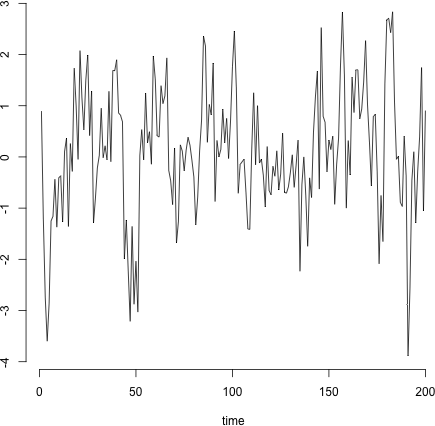
\includegraphics[width=.4\linewidth]{figure/hw1_Q4ts-1} }
\subfloat[Time Series of (4)\label{fig:Q4ts2}]{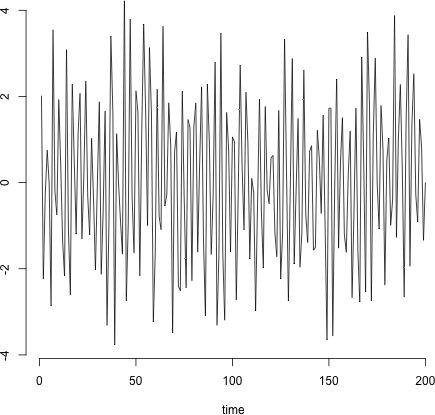
\includegraphics[width=.4\linewidth]{figure/hw1_Q4ts-2} }

}

\caption[200 observations from (3) and (4)]{200 observations from (3) and (4)}\label{fig:Q4ts}
\end{figure}


\end{knitrout}
		Figure \ref{fig:Q4ts} shows 200 observations from model \ref{M1} and \ref{M2} with model \ref{M1} parameters $\phi_1 = 0.5$, $\phi_2 = 0.15$ and $v = 1$ and model \ref{M2} parameters $a = 1$, $b = 2$ and $\omega_0 = 0.3$.
		
		\item Find the MLEs of the parameters in model (\ref{M1}) and (\ref{M2}). Use the conditional likelihood for model (\ref{M1}).\\
		\textbf{Solution:}\\
		Both models can be written in a matrix form of linear regression models, $\bfy = \bfF'\bsbeta + \bsep$ and because of Normality, the MLEs for the regression coefficients are OLS estimates, which is of form $\hat{\bsbeta} = (\bfF\bfF')^{-1}\bfF \bfy$. The ML estimate for $v$ is $R / n$, where $R = (\bfy - \bfF'\hat{\bsbeta})'(\bfy - \bfF'\hat{\bsbeta})$.


		Hence, given the generated data set, the ML estimate for $(\phi_1, \phi_2)$ are $(\hat{\phi}_{1, MLE}, \hat{\phi}_{2, MLE}) = (0.51, 0.102)$. The MLE for $v$ of model (\ref{M1}) is $\hat{v}^{(1)}_{MLE} = 1.057$
		
		For model (\ref{M2}), the ML estimates are $(\hat{a}_{MLE}, \hat{b}_{MLE}) = (0.994, 2.044)$ and $\hat{v}^{(2)}_{MLE} = 0.965$.
		
		\item Find the MAP estimators of the model parameters under the reference prior. Again, use the conditional likelihood for model (\ref{M1}).\\
		\textbf{Solution:}\\


		Under reference prior, OLS estimates for $(\phi_1, \phi_2)$ and $(a, b)$ are also MAPs. Hence $(\hat{\phi}_{1, MAP}, \hat{\phi}_{2, MAP}) = (0.51, 0.102)$ and $(\hat{a}_{MAP}, \hat{b}_{MAP}) = (0.994, 2.044)$. From Problem 2, we learn that $(v|\mathbf{y, F}) \sim IG\left( \frac{n-2}{2}, \frac{(n-2)s^2}{2} \right)$. Hence the MAP for $v$ is $R / n$, and so  $\hat{v}^{(1)}_{MAP} = 1.057$ and  $\hat{v}^{(2)}_{MAP} = 0.965$.
		
		\item Sketch $p(v|y_{1:n})$ and $p(\phi _1, \phi _2 | y_{1:n})$ for model (\ref{M1}).\\
		\textbf{Solution:}
%		<<Q4d1v, dev = 'tikz', fig.pos='h', cache=FALSE>>=
%		@
%		<<Q4d1phi, h = 2>>=
%		@
		Please see Figure \ref{fig:Q4d}.
\begin{knitrout}
\definecolor{shadecolor}{rgb}{0.969, 0.969, 0.969}\color{fgcolor}\begin{figure}[h]

{\centering \subfloat[Marginals of $v$\label{fig:Q4d1}]{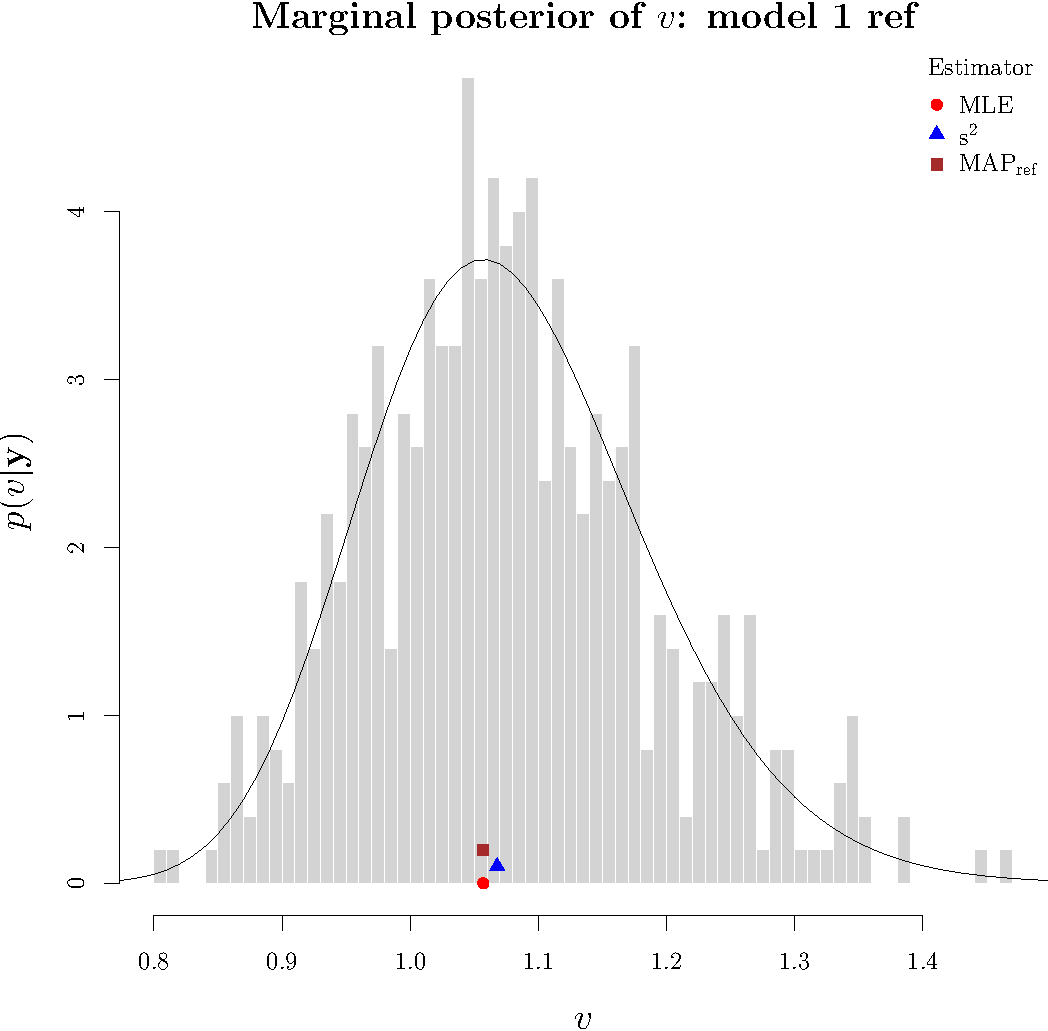
\includegraphics[width=.4\linewidth]{figure/hw1_Q4d-1} }
\subfloat[Marginals of $(\phi_1, \phi_2)$\label{fig:Q4d2}]{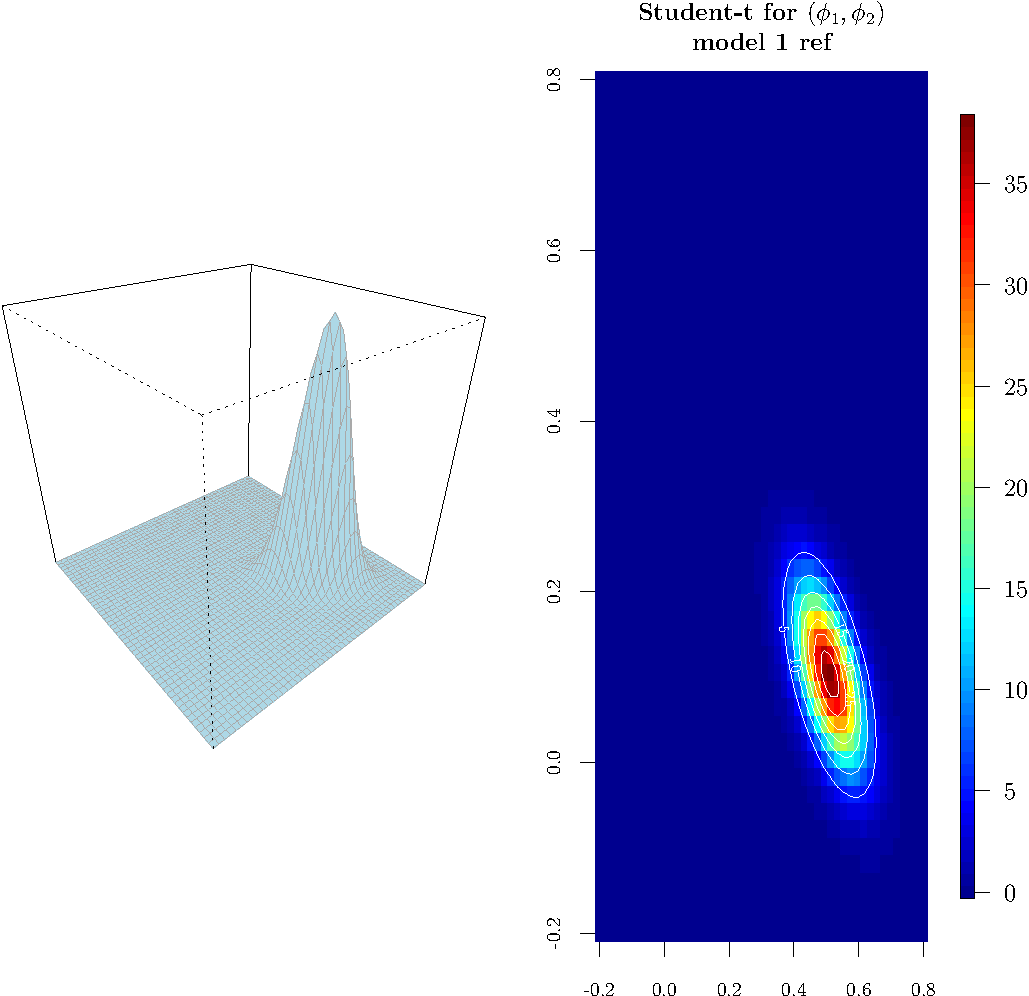
\includegraphics[width=.4\linewidth]{figure/hw1_Q4d-2} }

}

\caption[Marginals of $v$ and $(\phi_1, \phi_2)$ of model (\ref{M1}) under reference prior]{Marginals of $v$ and $(\phi_1, \phi_2)$ of model (\ref{M1}) under reference prior}\label{fig:Q4d}
\end{figure}


\end{knitrout}
%		<<tikz, tidy.opts=list(width.cutoff=40), dev='tikz'>>=
%		# tidy.opts=list(width.cutoff=40), dev='tikz'
%		library(tikzDevice)
%		plot(0, type = "n", ann = FALSE)
%		text(0, paste("$p(\\theta|\\mathbf{x})", "\\propto",
%		"\\pi(\\theta)f(\\mathbf{x}|\\theta)$"), cex = 2)
%		@
		\item Sketch $p(a, b|y_{1:n})$ and $p(a|y_{1:n})$ in model (\ref{M2}).\\
		\textbf{Solution:}\\
		Please see Figure \ref{fig:Q4e2}.
\begin{knitrout}
\definecolor{shadecolor}{rgb}{0.969, 0.969, 0.969}\color{fgcolor}\begin{figure}[h]

{\centering \subfloat[Marginals of $v$\label{fig:Q4e21}]{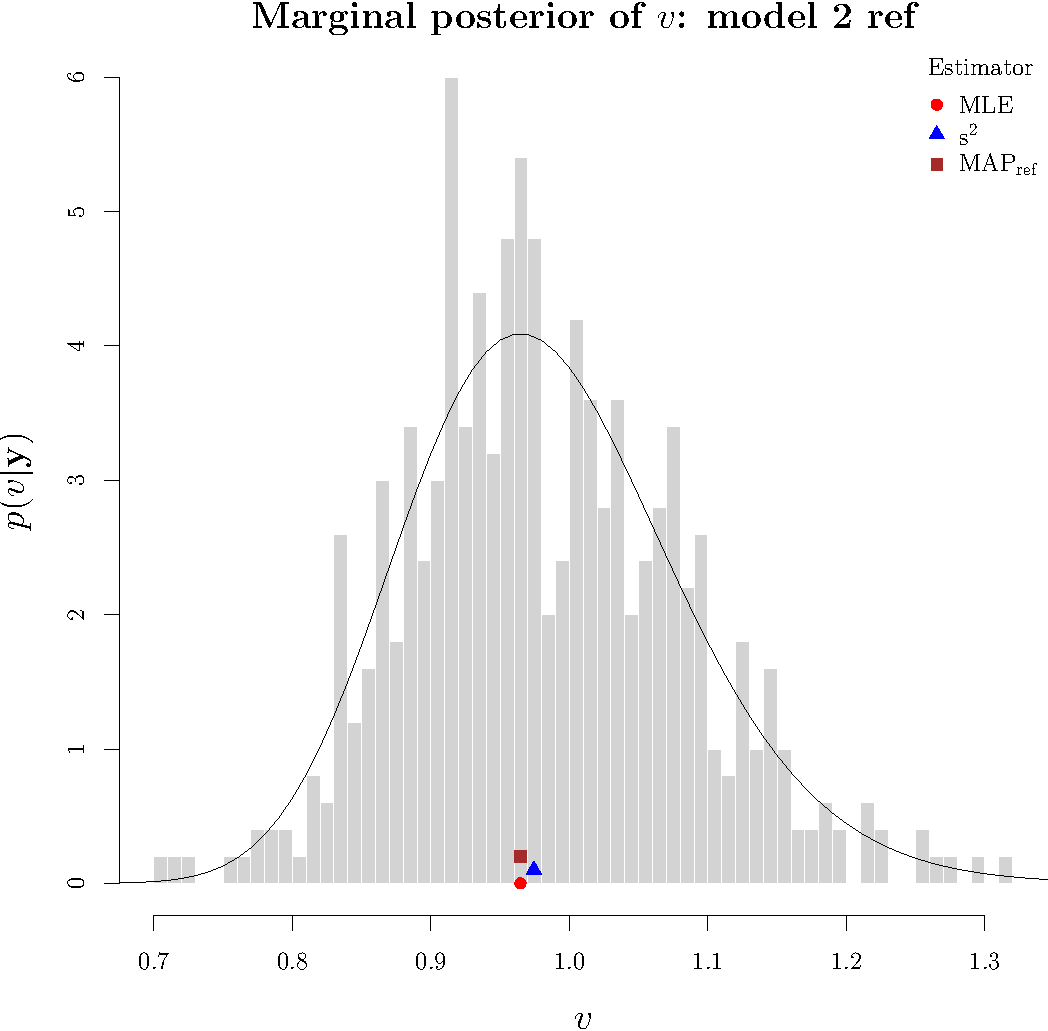
\includegraphics[width=.4\linewidth]{figure/hw1_Q4e2-1} }
\subfloat[Marginals of $(a, b)$\label{fig:Q4e22}]{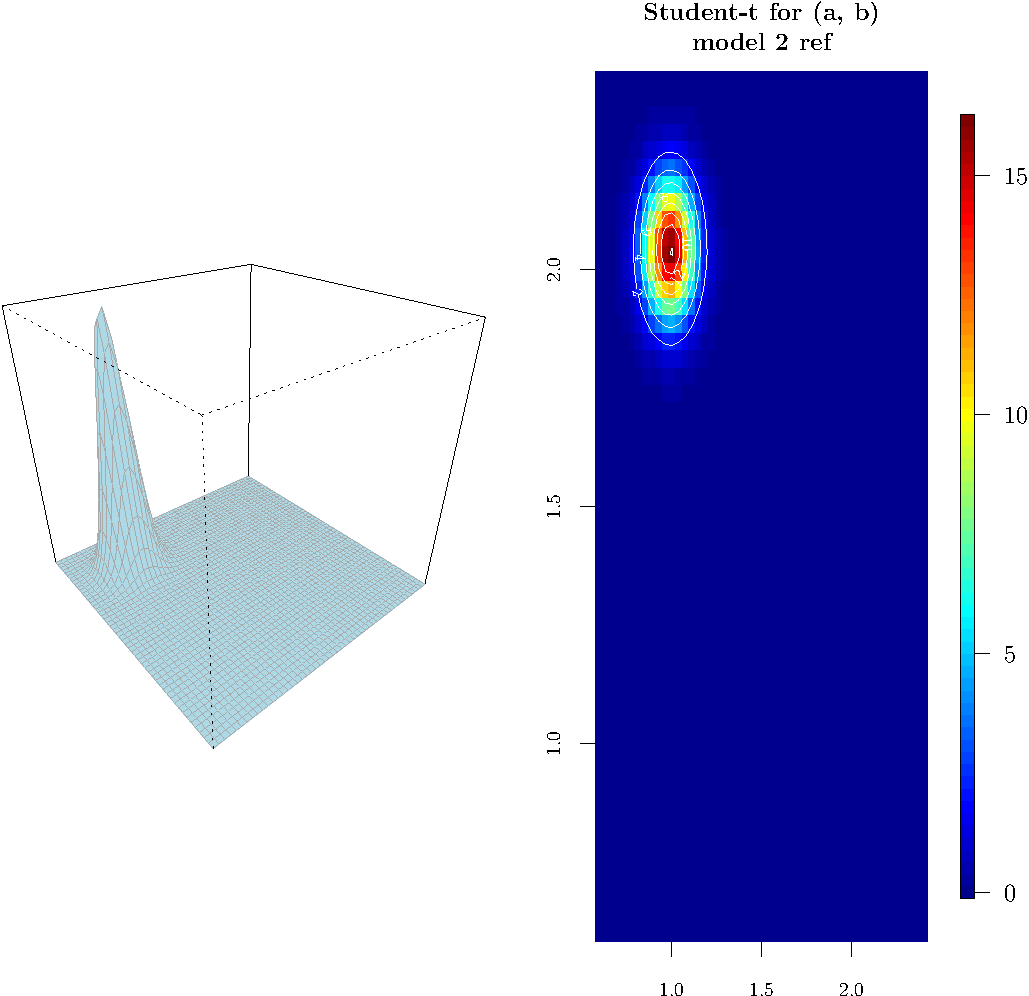
\includegraphics[width=.4\linewidth]{figure/hw1_Q4e2-2} }

}

\caption[Marginals of $v$ and $(a, b)$ of model (\ref{M2}) under reference prior]{Marginals of $v$ and $(a, b)$ of model (\ref{M2}) under reference prior}\label{fig:Q4e2}
\end{figure}


\end{knitrout}
		
		\item Perform a conjugate Bayesian analysis, i.e., repeat (c) to (e) assuming conjugate prior distributions in both models. Study the sensitivity of the posterior distributions to the choice of the hyperparameters in the prior.\\
		\textbf{Solution:}\\


		For model 1, with the prior $(\phi_1, \phi_2)' \sim N_2(\mathbf{m_0}, \mathbf{C_0})$, where $\mathbf{m_0} = (0.2, -0.5)$ and $\mathbf{C_0} = diag(3, 3)$ and $v \sim IG(n_0, d_0)$ where $n_0 = 10$ and $d_0 = 20$, we have $(\hat{\phi}_{1, MAPconj}, \hat{\phi}_{2, MAPconj}) = (0.51, 0.102)$ and $\hat{v} _{MAPconj}^{(1)} = 1.093$.
		
		For model 2, we use prior $(a, b)' \sim N_2(\mathbf{m_0}, \mathbf{C_0})$, where $\mathbf{m_0} = (2, 3)$ and $\mathbf{C_0} = diag(1, 2)$ and $v \sim IG(n_0, d_0)$ where $n_0 = 10$ and $d_0 = 20$. Under this setting, we have $(\hat{a}_{1, MAPconj}, \hat{b}_{2, MAPconj}) = (1.004, 2.053)$ and $\hat{v} _{MAPconj}^{(2)} = 1.013$
		
		Please see Figure \ref{fig:Q4f1d} and Figure \ref{fig:Q4f2e} for marginals under conjugate priors.
		
\begin{knitrout}
\definecolor{shadecolor}{rgb}{0.969, 0.969, 0.969}\color{fgcolor}\begin{figure}[h]

{\centering \subfloat[Marginals of $v$\label{fig:Q4f1d1}]{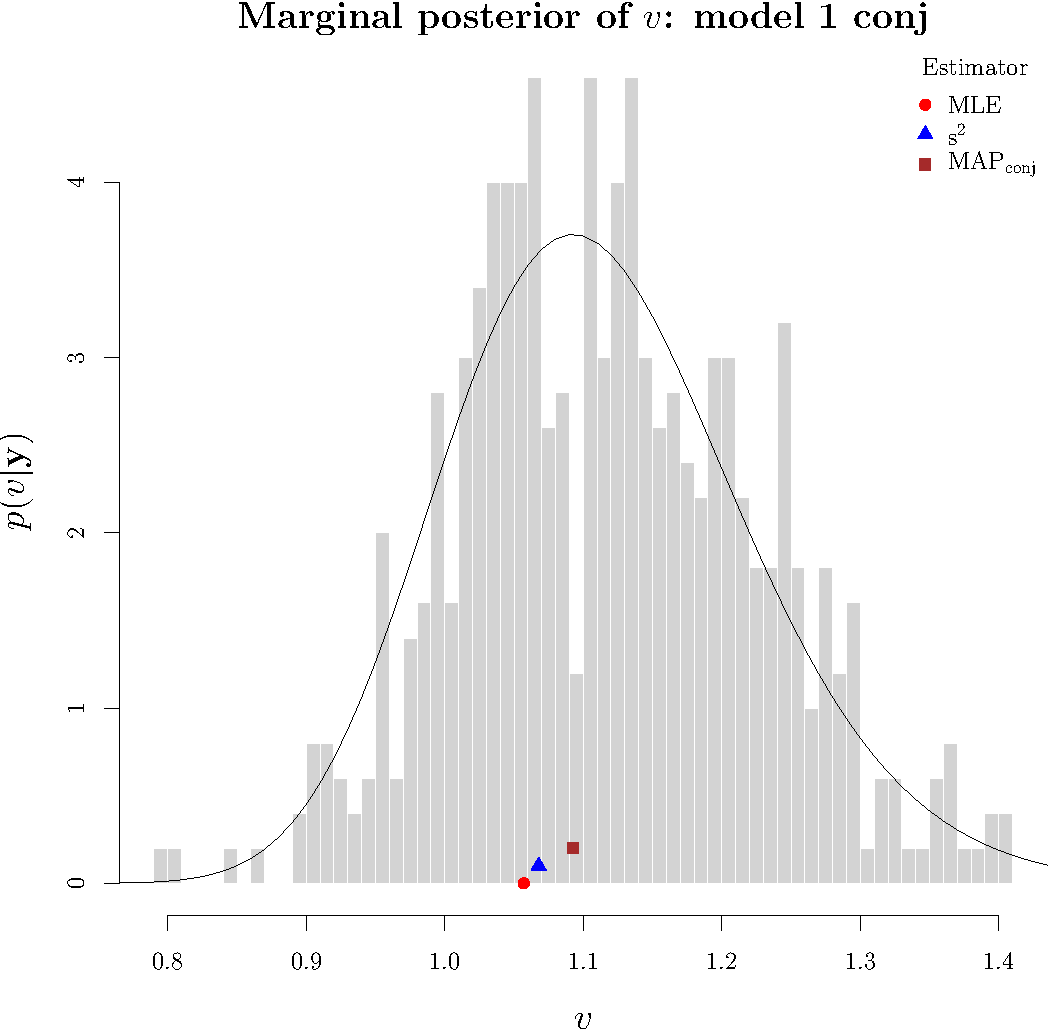
\includegraphics[width=.4\linewidth]{figure/hw1_Q4f1d-1} }
\subfloat[Marginals of $(\phi_1, \phi_2)$\label{fig:Q4f1d2}]{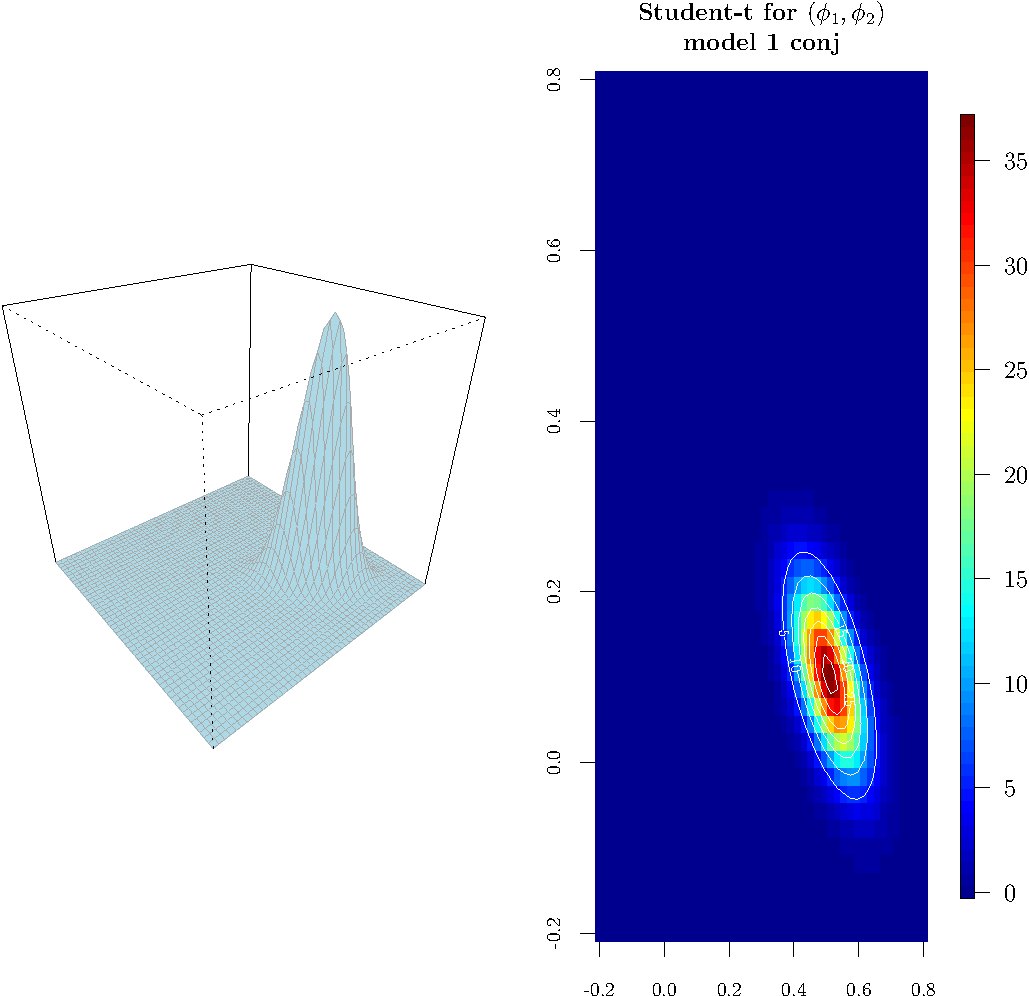
\includegraphics[width=.4\linewidth]{figure/hw1_Q4f1d-2} }

}

\caption[Marginals of $v$ and $(\phi_1, \phi_2)$ of model (\ref{M1}) under conjugate prior]{Marginals of $v$ and $(\phi_1, \phi_2)$ of model (\ref{M1}) under conjugate prior}\label{fig:Q4f1d}
\end{figure}


\end{knitrout}
\begin{knitrout}
\definecolor{shadecolor}{rgb}{0.969, 0.969, 0.969}\color{fgcolor}\begin{figure}[h]

{\centering \subfloat[Marginals of $v$\label{fig:Q4f2e1}]{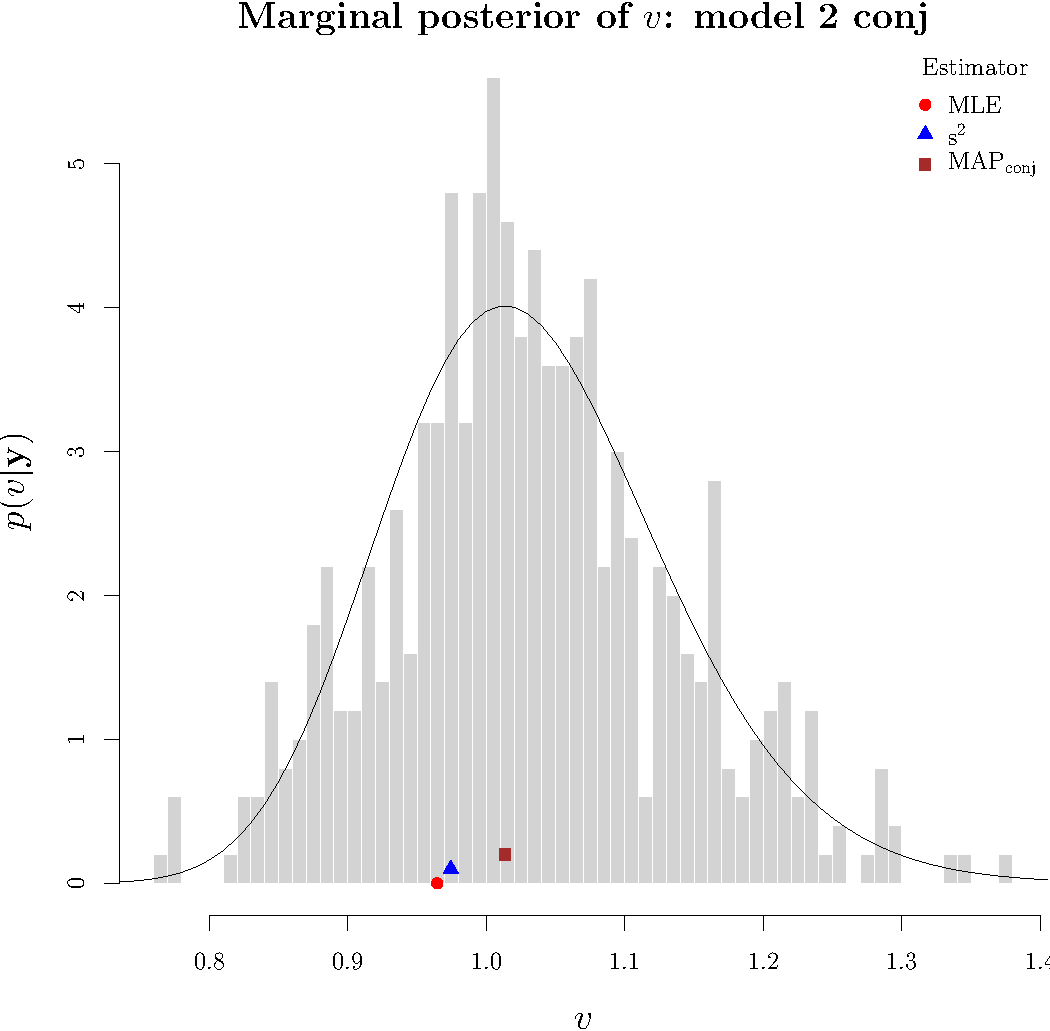
\includegraphics[width=.4\linewidth]{figure/hw1_Q4f2e-1} }
\subfloat[Marginals of $(a, b)$\label{fig:Q4f2e2}]{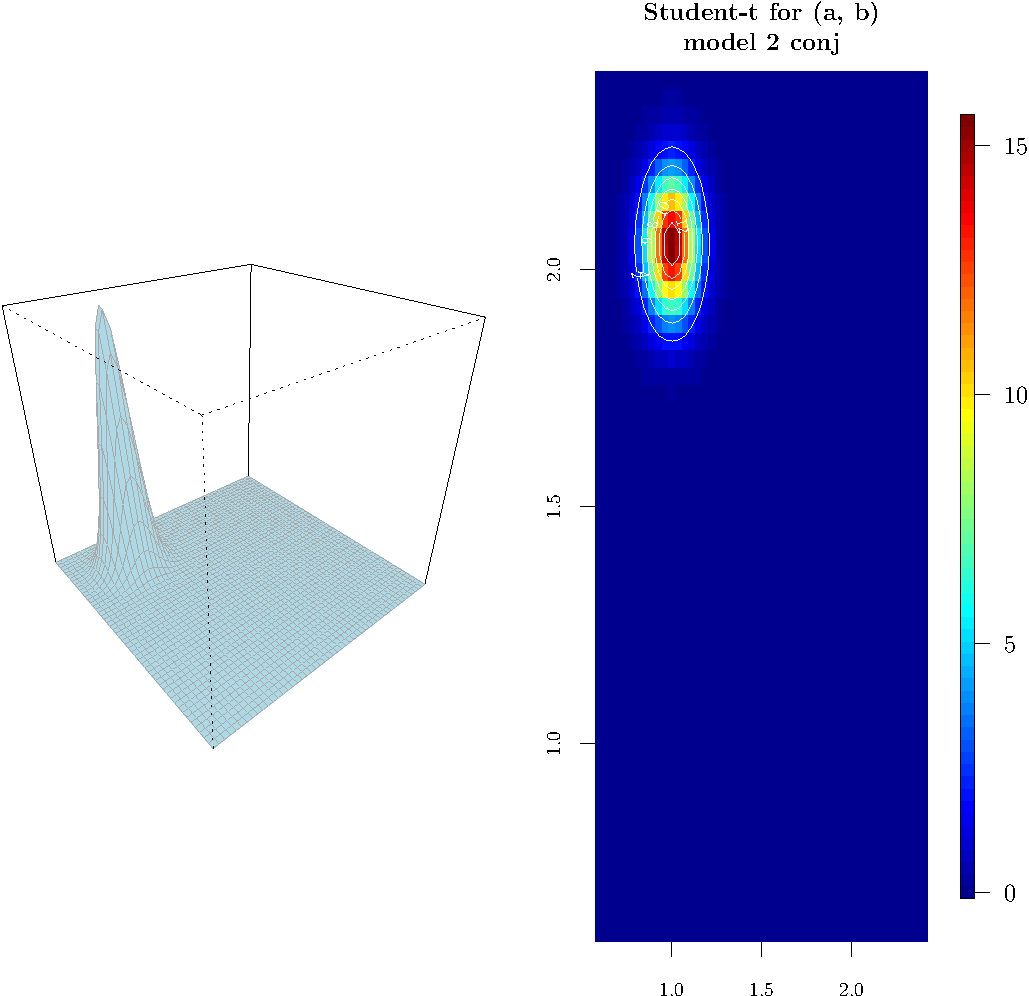
\includegraphics[width=.4\linewidth]{figure/hw1_Q4f2e-2} }

}

\caption[Marginals of $v$ and $(a, b)$ of model (\ref{M2}) under conjugate prior]{Marginals of $v$ and $(a, b)$ of model (\ref{M2}) under conjugate prior}\label{fig:Q4f2e}
\end{figure}


\end{knitrout}
		
		Sensitivity analysis can be seen in Figure \ref{fig:Q4f1senv}, \ref{fig:Q4f1senphi}, \ref{fig:Q4f2senv}, \ref{fig:Q4f2senab1} and \ref{fig:Q4f2senab2}.
		
\begin{knitrout}
\definecolor{shadecolor}{rgb}{0.969, 0.969, 0.969}\color{fgcolor}\begin{figure}

{\centering 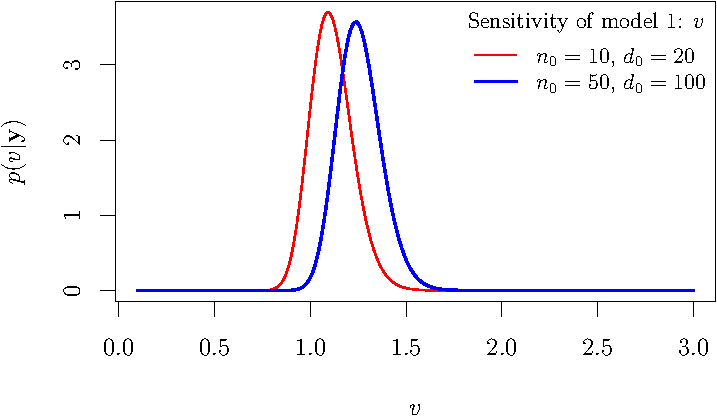
\includegraphics[width=.7\linewidth]{figure/hw1_Q4f1senv-1} 

}

\caption[Marginal posterior of $v$ of model 1, sensitivity]{Marginal posterior of $v$ of model 1, sensitivity.}\label{fig:Q4f1senv}
\end{figure}


\end{knitrout}
\begin{knitrout}
\definecolor{shadecolor}{rgb}{0.969, 0.969, 0.969}\color{fgcolor}\begin{figure}

{\centering 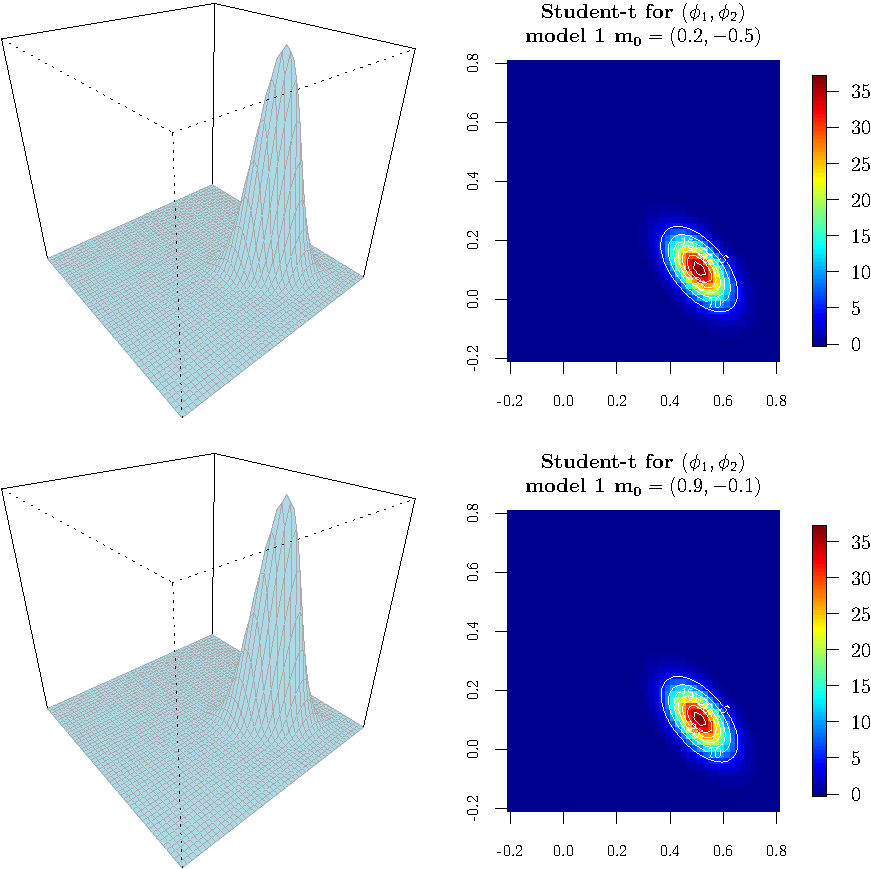
\includegraphics[width=.8\linewidth]{figure/hw1_Q4f1senphi-1} 

}

\caption[Marginal posterior of $(\phi_1, \phi_2)$ of model 1 with same prior of $v$, sensitivity]{Marginal posterior of $(\phi_1, \phi_2)$ of model 1 with same prior of $v$, sensitivity.}\label{fig:Q4f1senphi}
\end{figure}


\end{knitrout}
\begin{knitrout}
\definecolor{shadecolor}{rgb}{0.969, 0.969, 0.969}\color{fgcolor}\begin{figure}

{\centering 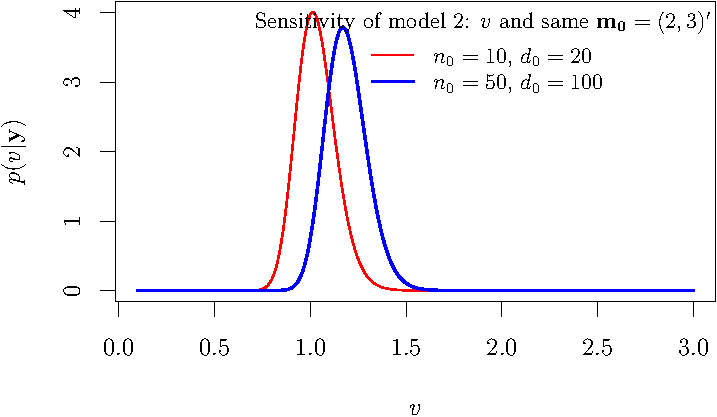
\includegraphics[width=.7\linewidth]{figure/hw1_Q4f2senv-1} 

}

\caption[Marginal posterior of $v$ of model 2, sensitivity]{Marginal posterior of $v$ of model 2, sensitivity.}\label{fig:Q4f2senv}
\end{figure}


\end{knitrout}
\begin{knitrout}
\definecolor{shadecolor}{rgb}{0.969, 0.969, 0.969}\color{fgcolor}\begin{figure}

{\centering 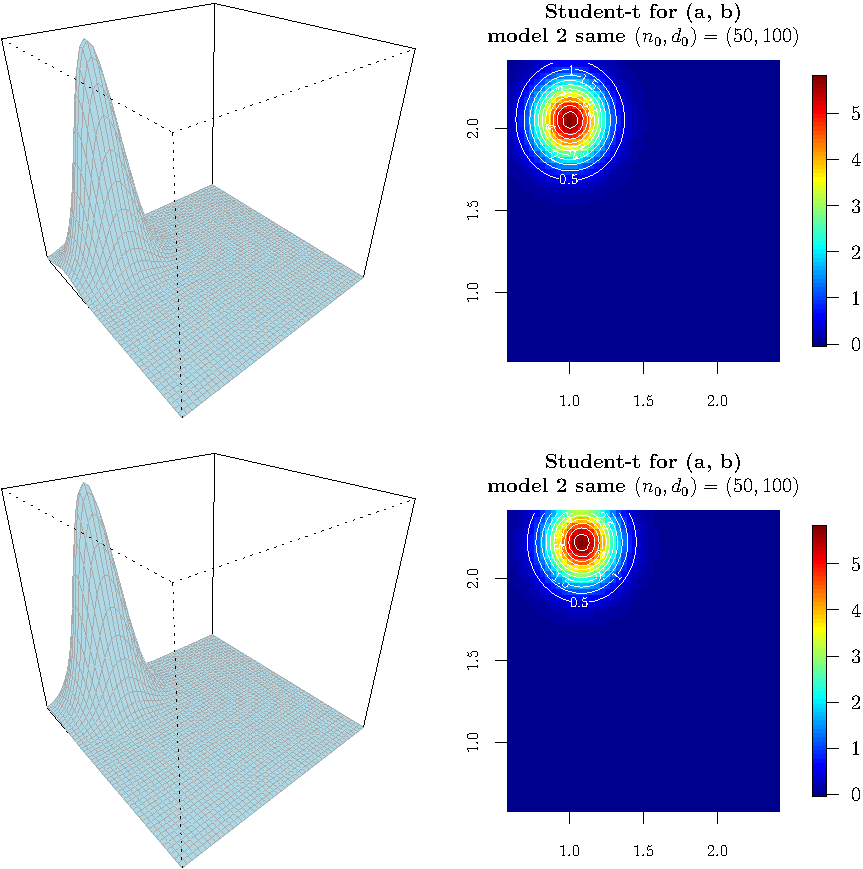
\includegraphics[width=.8\linewidth]{figure/hw1_Q4f2senab1-1} 

}

\caption[Marginal posterior of (a, b) of model 2 with the same prior on $v$ and different $\mathbf{m_0}$s, sensitivity]{Marginal posterior of (a, b) of model 2 with the same prior on $v$ and different $\mathbf{m_0}$s, sensitivity.}\label{fig:Q4f2senab1}
\end{figure}


\end{knitrout}
\begin{knitrout}
\definecolor{shadecolor}{rgb}{0.969, 0.969, 0.969}\color{fgcolor}\begin{figure}

{\centering 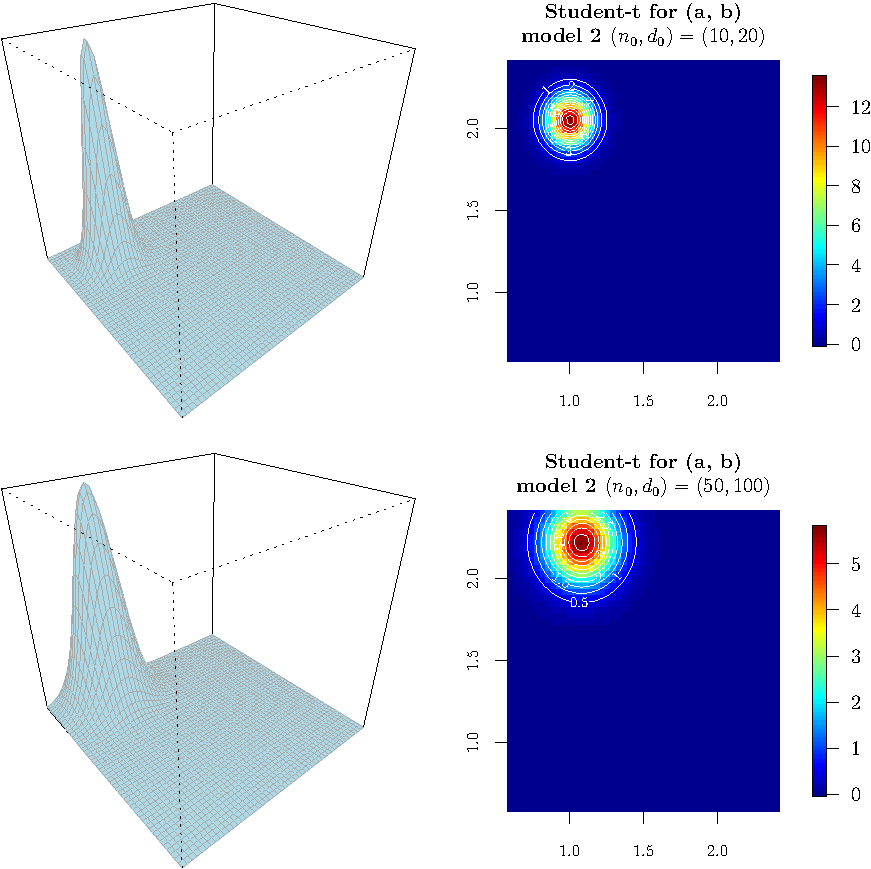
\includegraphics[width=.8\linewidth]{figure/hw1_Q4f2senab2-1} 

}

\caption[Marginal posterior of (a, b) of model 2 with different priors on $v$ and different $\mathbf{m_0}$s, sensitivity]{Marginal posterior of (a, b) of model 2 with different priors on $v$ and different $\mathbf{m_0}$s, sensitivity.}\label{fig:Q4f2senab2}
\end{figure}


\end{knitrout}
		
	\end{enumerate}
		
	\item \textbf{Chapter 2 Problem 7} Sample 1000 observations from the model (1.1). Using a prior distribution of the form $p(\phi^{(i)}) = N(m, c)$, for some $c$ and $i = 1, 2$, $p(\theta) = U(\theta|-a, a)$ and $p(v) = IG(\alpha _0, \beta _0)$, obtain samples from the joint posterior distribution by implementing a Metropolis-Hasting algorithm.\\
	\textbf{Solution:}

	\begin{figure}
\begin{knitrout}
\definecolor{shadecolor}{rgb}{0.969, 0.969, 0.969}\color{fgcolor}

{\centering 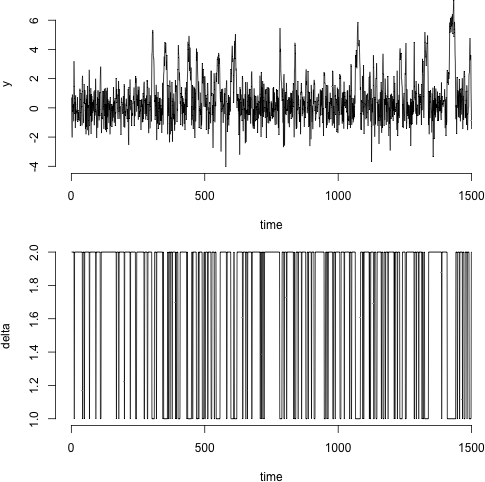
\includegraphics[width=0.49\linewidth]{figure/hw1_Q5a_plot-1} 

}



\end{knitrout}
		\caption{1000 time series observations of $y$ and $\delta$ from the model (1.1).}
		\label{Q5a_plot}
	\end{figure}

	First, we sample 1000 observations from the model (1.1). The $y$ and $\delta$ series shown in Figure \ref{Q5a_plot} look good.
	

	\begin{figure}
\begin{knitrout}
\definecolor{shadecolor}{rgb}{0.969, 0.969, 0.969}\color{fgcolor}

{\centering 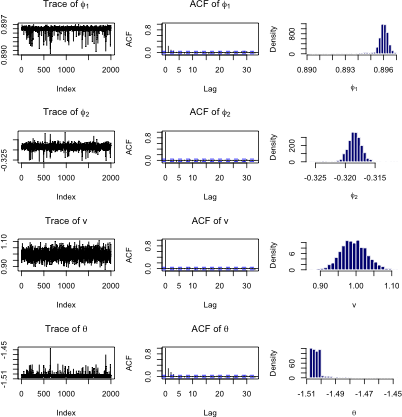
\includegraphics[width=.8\linewidth]{figure/hw1_Q5MCMCplot-1} 

}



\end{knitrout}
		\caption{Trace plots, ACFs and histograms of $\phi_1$, $\phi_2$, $v$ and $\theta$.}
		\label{Q5MCMCplot}
	\end{figure}
	
	We can derive full conditionals for $\phi_1$, $\phi_2$ and $v$, and perform Metropolis-Hastings step on $\theta$. A Gaussian random walk proposal is used and the variance is tuned to have reasonable acceptance rate.
	
	We use 21000 iterations, burn the first 1000 draws and thin the sequence by keeping every 10th draw and discarding the rest. Therefore, 2000 draws are stored for analysis. 
	
	Initial values are $\phi_1^{(0)} = 0.5$, $\phi_2^{(0)} = \ensuremath{-0.5}$, $\theta^{(0)} = \ensuremath{-2}$ and $v^{(0)} = 2$
	
	Hyperparameters are chosen to be $m = 0$, $c = 1$, $a = 3$, $\alpha_0 = 3$ and $\beta_0 = 0.003$.
	
% latex table generated in R 3.3.1 by xtable 1.8-2 package
% Fri Sep 23 12:04:43 2016
\begin{table}[ht]
\centering
\begin{tabular}{rrrrr}
  \hline
 & effective size & post. mean & 2.5\% quantile & 97.5\% quantile \\ 
  \hline
$\phi_1$ & 1101.40 & 0.90 & 0.89 & 0.90 \\ 
  $\phi_2$ & 2000.00 & -0.32 & -0.32 & -0.32 \\ 
  $v$ & 2000.00 & 0.99 & 0.93 & 1.07 \\ 
  $\theta$ & 967.63 & -1.50 & -1.51 & -1.49 \\ 
   \hline
\end{tabular}
\caption{Posterior Summary} 
\label{MCMCresult}
\end{table}

	
	Table \ref{MCMCresult} summarizes the posterior sample and Figure \ref{Q5MCMCplot} shows trace plots, ACFs and histograms of the parameters from the 2000 draws. 
\end{enumerate}



the R package \emph{knitr}

\citep{R-knitr}. It also relied on the R packages

\emph{ggplot2} \citep{R-coda} and \citep{R-repmis} and \citep{R-fields}.

The document can be completely reproduced from

source files available on GitHub at:

\url{https://GitHub.com/christophergandrud/Rep-Res-Examples}.

\clearpage
\newpage
\newpage
\section{Code}
\begin{knitrout}
\definecolor{shadecolor}{rgb}{0.969, 0.969, 0.969}\color{fgcolor}\begin{kframe}
\begin{alltt}
\hlcom{#### Global options}
\hlcom{# options(replace.assign=TRUE,width=90)}
\hlcom{# A penalty to be applied when deciding to print numeric values in fixed }
\hlcom{# or exponential notation}
\hlkwd{options}\hlstd{(}\hlkwc{scipen} \hlstd{=} \hlnum{1}\hlstd{,} \hlkwc{digits} \hlstd{=} \hlnum{3}\hlstd{,} \hlkwc{width} \hlstd{=} \hlnum{55}\hlstd{)}

\hlcom{#### Set chunk options}
\hlcom{# figure options}
\hlkwd{library}\hlstd{(knitr)}
\hlstd{opts_chunk}\hlopt{$}\hlkwd{set}\hlstd{(}\hlkwc{fig.path}\hlstd{=}\hlstr{'figure/hw1_'}\hlstd{,} \hlkwc{fig.align}\hlstd{=}\hlstr{'center'}\hlstd{,} \hlkwc{crop} \hlstd{=} \hlnum{TRUE}\hlstd{,}
               \hlkwc{dev} \hlstd{=} \hlstr{'png'}\hlstd{,} \hlkwc{out.width} \hlstd{=} \hlstr{"0.49\textbackslash{}\textbackslash{}linewidth"}\hlstd{)}

\hlcom{# error message options}
\hlstd{opts_chunk}\hlopt{$}\hlkwd{set}\hlstd{(}\hlkwc{warning} \hlstd{=} \hlnum{FALSE}\hlstd{,} \hlkwc{message} \hlstd{=} \hlnum{FALSE}\hlstd{,} \hlkwc{error} \hlstd{=} \hlnum{FALSE}\hlstd{)}
\hlcom{# other options: }
\hlcom{# the width of source code}
\hlcom{# changes in comments won't aff3ect the cache}
\hlstd{opts_chunk}\hlopt{$}\hlkwd{set}\hlstd{(}\hlkwc{tidy.opts} \hlstd{=} \hlkwd{list}\hlstd{(}\hlkwc{width.cutoff} \hlstd{=} \hlnum{65}\hlstd{),}
               \hlkwc{cache.comments} \hlstd{=} \hlnum{FALSE}\hlstd{,} \hlkwc{echo} \hlstd{=} \hlnum{FALSE}\hlstd{)}

\hlcom{#### Set hooks}
\hlcom{# set margin like margin = c(2, 3, 1, 1)}
\hlstd{knit_hooks}\hlopt{$}\hlkwd{set}\hlstd{(}\hlkwc{margin} \hlstd{=} \hlkwa{function}\hlstd{(}\hlkwc{before}\hlstd{,} \hlkwc{options}\hlstd{,} \hlkwc{envir}\hlstd{) \{}
        \hlkwa{if} \hlstd{(before) \{}
                \hlstd{m} \hlkwb{<-} \hlstd{options}\hlopt{$}\hlstd{margin}
                \hlkwa{if} \hlstd{(}\hlkwd{is.numeric}\hlstd{(m)} \hlopt{&&} \hlkwd{length}\hlstd{(m)} \hlopt{==} \hlnum{4L}\hlstd{) \{}
                        \hlkwd{par}\hlstd{(}\hlkwc{mar} \hlstd{= m)}
                \hlstd{\}}
        \hlstd{\}} \hlkwa{else NULL}
\hlstd{\})}
\hlcom{# crop = TRUE to crop the white margin}
\hlstd{knit_hooks}\hlopt{$}\hlkwd{set}\hlstd{(}\hlkwc{crop} \hlstd{= hook_pdfcrop)}
\hlcom{#### Set up aliases for chink options}
\hlkwd{set_alias}\hlstd{(}\hlkwc{w} \hlstd{=} \hlstr{"fig.width"}\hlstd{,} \hlkwc{h} \hlstd{=} \hlstr{"fig.height"}\hlstd{)}

\hlcom{#### Option templates}
\hlstd{opts_template}\hlopt{$}\hlkwd{set}\hlstd{(}
\hlkwc{fig.large} \hlstd{=} \hlkwd{list}\hlstd{(}\hlkwc{fig.width} \hlstd{=} \hlnum{7}\hlstd{,} \hlkwc{fig.height} \hlstd{=} \hlnum{5}\hlstd{),}
\hlkwc{fig.small} \hlstd{=} \hlkwd{list}\hlstd{(}\hlkwc{fig.width} \hlstd{=} \hlnum{3.5}\hlstd{,} \hlkwc{fig.height} \hlstd{=} \hlnum{3}\hlstd{)}
\hlstd{)}

\hlcom{#### Set the theme}
\hlcom{# thm <- knit_theme$get("bclear")}
\hlcom{# thm$background}
\hlcom{# thm$foreground}
\hlcom{# knit_theme$set(thm)}
\hlcom{# opts_chunk$set(background = "#f5f5f5")}

\hlcom{#### Load and cite R packages}
\hlcom{# List of packages}
\hlstd{PackageUsed} \hlkwb{<-} \hlkwd{c}\hlstd{(}\hlstr{"knitr"}\hlstd{,} \hlstr{"pscl"}\hlstd{,} \hlstr{"coda"}\hlstd{,} \hlstr{"parallel"}\hlstd{,}
\hlstr{"doParallel"}\hlstd{,} \hlstr{"tikzDevice"}\hlstd{,} \hlstr{"mvtnorm"}\hlstd{,} \hlstr{"fields"}\hlstd{,} \hlstr{"repmis"}\hlstd{)}
\hlcom{# Load packages}
\hlkwd{lapply}\hlstd{(PackageUsed, library,} \hlkwc{character.only} \hlstd{=} \hlnum{TRUE}\hlstd{)}

\hlcom{#### Read external R scripts}
\hlkwd{read_chunk}\hlstd{(}\hlstr{"../Analysis/AMS223_HW1_P1.R"}\hlstd{)}
\hlkwd{read_chunk}\hlstd{(}\hlstr{'../Analysis/AMS223_HW1_P4.R'}\hlstd{)}
\hlkwd{read_chunk}\hlstd{(}\hlstr{'../Analysis/AMS223_HW1_P5.R'}\hlstd{)}
\hlkwd{read_chunk}\hlstd{(}\hlstr{'../Analysis/AMS_223_HW1_Q6.R'}\hlstd{)}
\hlcom{# acceptance rate}
\hlstd{accept_rate} \hlkwb{=} \hlstd{mcmc_sample}\hlopt{$}\hlstd{accept} \hlopt{/} \hlstd{mcmc_sample}\hlopt{$}\hlstd{count}

\hlstd{quan025} \hlkwb{<-} \hlkwa{function}\hlstd{(}\hlkwc{x}\hlstd{) \{}
    \hlkwd{quantile}\hlstd{(x,} \hlkwc{prob} \hlstd{=} \hlnum{0.025}\hlstd{)}
\hlstd{\}}
\hlstd{quan975} \hlkwb{<-} \hlkwa{function}\hlstd{(}\hlkwc{x}\hlstd{) \{}
    \hlkwd{quantile}\hlstd{(x,} \hlkwc{prob} \hlstd{=} \hlnum{0.975}\hlstd{)}
\hlstd{\}}

\hlkwd{library}\hlstd{(coda)}
\hlcom{# draws <- cbind(Phi1, Phi2, V, Theta)[sampleidx, ]}
\hlkwd{colnames}\hlstd{(draws)} \hlkwb{<-} \hlkwd{c}\hlstd{(}\hlstr{"$\textbackslash{}\textbackslash{}phi_1$"}\hlstd{,} \hlstr{"$\textbackslash{}\textbackslash{}phi_2$"}\hlstd{,} \hlstr{"$v$"}\hlstd{,} \hlstr{"$\textbackslash{}\textbackslash{}theta$"}\hlstd{)}
\hlstd{result} \hlkwb{<-} \hlkwd{round}\hlstd{(}\hlkwd{cbind}\hlstd{(}\hlkwd{apply}\hlstd{(draws,} \hlnum{2}\hlstd{, effectiveSize),}
                      \hlkwd{apply}\hlstd{(draws,} \hlnum{2}\hlstd{, mean),}
                      \hlkwd{apply}\hlstd{(draws,} \hlnum{2}\hlstd{, quan025),}
                      \hlkwd{apply}\hlstd{(draws,} \hlnum{2}\hlstd{, quan975)),} \hlnum{4}\hlstd{)}
\hlkwd{colnames}\hlstd{(result)} \hlkwb{<-} \hlkwd{c}\hlstd{(}\hlstr{"effective size"}\hlstd{,} \hlstr{"post. mean"}\hlstd{,} \hlstr{"2.5% quantile"}\hlstd{,}
                      \hlstr{"97.5% quantile"}\hlstd{)}
\hlkwd{library}\hlstd{(xtable)}
\hlkwd{print}\hlstd{(}\hlkwd{xtable}\hlstd{(result,} \hlkwc{caption} \hlstd{=} \hlstr{"Posterior Summary"}\hlstd{,} \hlkwc{label} \hlstd{=} \hlstr{"MCMCresult"}\hlstd{),}
      \hlkwc{sanitize.rownames.function}\hlstd{=}\hlkwa{function}\hlstd{(}\hlkwc{x}\hlstd{)\{x\})}
\hlcom{# for html output}
\hlcom{# print(xtable(result, caption = "Posterior Summary", label = "MCMCresult"),}
\hlcom{#       sanitize.rownames.function=function(x)\{x\}, type = "html")}
\hlcom{# AMS 223 Time Series }
\hlcom{# Cheng-Han Yu, Dept of Applied Math and Statistics, UC Santa Cruz}
\hlcom{# HW1 Time series and Baysian inference overview}
\hlcom{# Problem 1: Chap 1 problem 2}
\hlstd{phi} \hlkwb{<-} \hlnum{0.9}
\hlstd{v} \hlkwb{<-} \hlnum{1}
\hlstd{y0} \hlkwb{<-} \hlnum{0.1}
\hlstd{n} \hlkwb{<-} \hlnum{100}
\hlstd{y} \hlkwb{<-} \hlkwd{rep}\hlstd{(}\hlnum{NA}\hlstd{, n)}
\hlcom{# y[1] <- y0}
\hlkwd{set.seed}\hlstd{(}\hlnum{123456}\hlstd{)}
\hlkwa{for} \hlstd{(i} \hlkwa{in} \hlnum{1}\hlopt{:}\hlstd{n) \{}
    \hlkwa{if} \hlstd{(i} \hlopt{==} \hlnum{1}\hlstd{) \{}
        \hlstd{y[i]} \hlkwb{<-} \hlstd{phi} \hlopt{*} \hlstd{y0} \hlopt{+} \hlkwd{rnorm}\hlstd{(}\hlnum{1}\hlstd{,} \hlnum{0}\hlstd{, v)}
    \hlstd{\}} \hlkwa{else} \hlstd{\{}
        \hlstd{y[i]} \hlkwb{<-} \hlstd{phi} \hlopt{*} \hlstd{y[i} \hlopt{-} \hlnum{1}\hlstd{]} \hlopt{+} \hlkwd{rnorm}\hlstd{(}\hlnum{1}\hlstd{,} \hlnum{0}\hlstd{, v)}
    \hlstd{\}}
\hlstd{\}}
\hlcom{# (a) MLE for conditional likelihood can be derived analytically}
\hlstd{ym1} \hlkwb{<-} \hlstd{y[}\hlopt{-}\hlstd{n]}
\hlstd{yt} \hlkwb{<-} \hlstd{y[}\hlopt{-}\hlnum{1}\hlstd{]}
\hlstd{phi_cmle} \hlkwb{<-} \hlkwd{sum}\hlstd{(yt} \hlopt{*} \hlstd{ym1)} \hlopt{/} \hlstd{(}\hlkwd{sum}\hlstd{(ym1} \hlopt{^} \hlnum{2}\hlstd{))}
\hlstd{v_cmle} \hlkwb{<-} \hlkwd{sum}\hlstd{((yt} \hlopt{-} \hlstd{phi_cmle} \hlopt{*} \hlstd{ym1)} \hlopt{^} \hlnum{2}\hlstd{)} \hlopt{/} \hlstd{(n} \hlopt{-} \hlnum{1}\hlstd{)}
\hlcom{# (b) MLE for the unconditional likelihood using Newton-Raphson method }
\hlcom{# Simulation data from AR(1) with phi = 0.9, v = 1 and y0 = 0.1 }
\hlcom{# with sample size n}

\hlcom{# Newton-Raphson iteration starting value}
\hlstd{phi0} \hlkwb{<-} \hlnum{0.8}
\hlstd{v0} \hlkwb{<-} \hlnum{0.8}
\hlstd{theta0} \hlkwb{<-} \hlkwd{c}\hlstd{(phi0, v0)}
\hlcom{# Hessian(theta0[1], theta0[2])}
\hlcom{# solve(Hessian(theta0[1], theta0[2]))}
\hlcom{# gradient of the objective function (1.17)}
\hlstd{Qstar} \hlkwb{<-} \hlstd{y[}\hlnum{1}\hlstd{]} \hlopt{^} \hlnum{2} \hlopt{*} \hlstd{(}\hlnum{1} \hlopt{-} \hlstd{phi} \hlopt{^} \hlnum{2}\hlstd{)} \hlopt{+} \hlkwd{sum}\hlstd{((yt} \hlopt{-} \hlstd{phi} \hlopt{*} \hlstd{ym1)} \hlopt{^} \hlnum{2}\hlstd{)}
\hlstd{gradient} \hlkwb{<-} \hlkwa{function}\hlstd{(}\hlkwc{phi}\hlstd{,} \hlkwc{v}\hlstd{) \{}
    \hlstd{dphi} \hlkwb{<-} \hlstd{(}\hlopt{-}\hlnum{2} \hlopt{*} \hlstd{phi} \hlopt{/} \hlstd{(}\hlnum{1} \hlopt{-} \hlstd{phi} \hlopt{^} \hlnum{2}\hlstd{))} \hlopt{+} \hlstd{(}\hlnum{2} \hlopt{/} \hlstd{v)} \hlopt{*}
        \hlstd{(y[}\hlnum{1}\hlstd{]} \hlopt{^} \hlnum{2} \hlopt{*} \hlstd{phi} \hlopt{+} \hlkwd{sum}\hlstd{(yt} \hlopt{*} \hlstd{ym1)} \hlopt{-} \hlstd{phi} \hlopt{*} \hlkwd{sum}\hlstd{(ym1} \hlopt{^} \hlnum{2}\hlstd{))}
    \hlstd{dv} \hlkwb{<-} \hlstd{(}\hlopt{-}\hlstd{n} \hlopt{/} \hlstd{v)} \hlopt{+} \hlstd{(}\hlnum{1} \hlopt{/} \hlstd{v} \hlopt{^} \hlnum{2}\hlstd{)} \hlopt{*} \hlstd{Qstar}
    \hlkwd{return} \hlstd{(}\hlkwd{c}\hlstd{(dphi, dv))}
\hlstd{\}}

\hlcom{# Hessian of the objective function (1.17)}
\hlstd{Hessian} \hlkwb{<-} \hlkwa{function}\hlstd{(}\hlkwc{phi}\hlstd{,} \hlkwc{v}\hlstd{) \{}
    \hlstd{dphiphi} \hlkwb{<-} \hlstd{(}\hlopt{-}\hlnum{2} \hlopt{*} \hlstd{(}\hlnum{1} \hlopt{+} \hlstd{phi} \hlopt{^} \hlnum{2}\hlstd{)} \hlopt{/} \hlstd{((}\hlnum{1} \hlopt{-} \hlstd{phi} \hlopt{^} \hlnum{2}\hlstd{)} \hlopt{^} \hlnum{2}\hlstd{))} \hlopt{+}
        \hlstd{(}\hlnum{2} \hlopt{/} \hlstd{v)} \hlopt{*} \hlstd{(y[}\hlnum{1}\hlstd{]} \hlopt{^} \hlnum{2} \hlopt{-} \hlkwd{sum}\hlstd{(ym1} \hlopt{^} \hlnum{2}\hlstd{))}
    \hlstd{dvv} \hlkwb{<-} \hlstd{(n} \hlopt{/} \hlstd{(v} \hlopt{^} \hlnum{2}\hlstd{))} \hlopt{-} \hlstd{(}\hlnum{2} \hlopt{*} \hlstd{Qstar} \hlopt{/} \hlstd{(v} \hlopt{^} \hlnum{3}\hlstd{))}
    \hlstd{dphiv} \hlkwb{<-} \hlstd{(}\hlopt{-}\hlnum{2} \hlopt{/} \hlstd{v} \hlopt{^} \hlnum{2}\hlstd{)} \hlopt{*} \hlstd{(y[}\hlnum{1}\hlstd{]} \hlopt{^} \hlnum{2}\hlopt{*} \hlstd{phi} \hlopt{+} \hlkwd{sum}\hlstd{(yt} \hlopt{*} \hlstd{ym1)} \hlopt{-}
                                \hlstd{phi} \hlopt{*} \hlkwd{sum}\hlstd{(ym1} \hlopt{^} \hlnum{2}\hlstd{))}
    \hlkwd{return} \hlstd{(}\hlkwd{matrix}\hlstd{(}\hlkwd{c}\hlstd{(dphiphi, dphiv, dphiv, dvv),} \hlkwc{nrow} \hlstd{=} \hlnum{2}\hlstd{))}
\hlstd{\}}

\hlcom{# Newton-Raphson iteration}
\hlstd{theta1} \hlkwb{<-} \hlstd{theta0} \hlopt{-} \hlkwd{solve}\hlstd{(}\hlkwd{Hessian}\hlstd{(theta0[}\hlnum{1}\hlstd{], theta0[}\hlnum{2}\hlstd{]))} \hlopt
                                \hlkwd{gradient}\hlstd{(theta0[}\hlnum{1}\hlstd{], theta0[}\hlnum{2}\hlstd{])}
\hlstd{count} \hlkwb{<-} \hlnum{1}
\hlkwa{while} \hlstd{(}\hlkwd{sum}\hlstd{(theta1} \hlopt{-} \hlstd{theta0)} \hlopt{^} \hlnum{2} \hlopt{>} \hlnum{1e-8}\hlstd{)\{}
    \hlstd{theta0} \hlkwb{<-} \hlstd{theta1}
    \hlstd{theta1} \hlkwb{<-} \hlstd{theta0} \hlopt{-} \hlkwd{solve}\hlstd{(}\hlkwd{Hessian}\hlstd{(theta0[}\hlnum{1}\hlstd{], theta0[}\hlnum{2}\hlstd{]))} \hlopt
        \hlkwd{gradient}\hlstd{(theta0[}\hlnum{1}\hlstd{], theta0[}\hlnum{2}\hlstd{])}
    \hlstd{count} \hlkwb{<-} \hlstd{count} \hlopt{+} \hlnum{1}
    \hlkwd{cat}\hlstd{(}\hlstr{"Iteration = "}\hlstd{, count,} \hlstr{"\textbackslash{}n"}\hlstd{,} \hlkwc{sep} \hlstd{=} \hlstr{""}\hlstd{)}
    \hlkwd{cat}\hlstd{(}\hlstr{"The MLE for (phi, v) = ("}\hlstd{, theta1[}\hlnum{1}\hlstd{],} \hlstr{", "}\hlstd{, theta1[}\hlnum{2}\hlstd{],} \hlstr{")"}\hlstd{,} \hlstr{"\textbackslash{}n"}\hlstd{,}
        \hlkwc{sep} \hlstd{=} \hlstr{""}\hlstd{)}
\hlstd{\}}
\hlcom{################################################################################}
\hlcom{# AMS 223 Time Series }
\hlcom{# Cheng-Han Yu, Dept of Applied Math and Statistics, UC Santa Cruz}
\hlcom{# HW1 Time series and Baysian inference overview}
\hlcom{# Problem 4: Chap 1 problem 5}
\hlcom{################################################################################}
\hlcom{# (a) Sample 200 obs}
\hlstd{n} \hlkwb{<-} \hlnum{200}
\hlstd{v} \hlkwb{<-} \hlnum{1}
\hlcom{# choose model 1 parameters}
\hlstd{phi1} \hlkwb{<-} \hlnum{0.5}
\hlstd{phi2} \hlkwb{<-} \hlnum{0.15}
\hlcom{# (a.1) sample 200 obs from model 1}
\hlcom{# set.seed(1234)}
\hlstd{y} \hlkwb{<-} \hlstd{stats}\hlopt{::}\hlkwd{arima.sim}\hlstd{(}\hlkwc{n} \hlstd{= n,} \hlkwc{model} \hlstd{=} \hlkwd{list}\hlstd{(}\hlkwc{ar} \hlstd{=} \hlkwd{c}\hlstd{(phi1, phi2)),} \hlkwc{sd} \hlstd{= v)}
\hlcom{# head(y)}
\hlkwd{plot}\hlstd{(y,} \hlkwc{type} \hlstd{=} \hlstr{"l"}\hlstd{,} \hlkwc{xlab} \hlstd{=} \hlstr{"time"}\hlstd{,} \hlkwc{ylab} \hlstd{=} \hlstr{""}\hlstd{,} \hlkwc{axes} \hlstd{= F)}
\hlkwd{axis}\hlstd{(}\hlnum{1}\hlstd{)}
\hlkwd{axis}\hlstd{(}\hlnum{2}\hlstd{)}

\hlstd{a} \hlkwb{<-} \hlnum{1}
\hlstd{b} \hlkwb{<-} \hlnum{2}
\hlstd{w0} \hlkwb{<-} \hlnum{0.3}
\hlcom{# (a.2) sample 200 obs from model 2}
\hlstd{angle} \hlkwb{=} \hlnum{2} \hlopt{*} \hlstd{w0} \hlopt{*} \hlstd{pi} \hlopt{*} \hlnum{1}\hlopt{:}\hlstd{n}
\hlstd{x} \hlkwb{=} \hlstd{a} \hlopt{*} \hlkwd{cos}\hlstd{(angle)} \hlopt{+} \hlstd{b} \hlopt{*} \hlkwd{sin}\hlstd{(angle)} \hlopt{+} \hlkwd{rnorm}\hlstd{(n,} \hlnum{0}\hlstd{, v)}
\hlcom{# head(x)}
\hlkwd{plot}\hlstd{(x,} \hlkwc{type} \hlstd{=} \hlstr{"l"}\hlstd{,} \hlkwc{xlab} \hlstd{=} \hlstr{"time"}\hlstd{,} \hlkwc{ylab} \hlstd{=} \hlstr{""}\hlstd{,} \hlkwc{axes} \hlstd{= F)}
\hlkwd{axis}\hlstd{(}\hlnum{1}\hlstd{)}
\hlkwd{axis}\hlstd{(}\hlnum{2}\hlstd{)}
\hlcom{# (b) Find MLE}
\hlcom{# (b.1) MLE for model 1}
\hlstd{f1} \hlkwb{<-} \hlstd{y[}\hlopt{-}\hlkwd{c}\hlstd{(}\hlnum{1}\hlstd{, n)]}  \hlcom{# 1st col of F'}
\hlstd{f2} \hlkwb{<-} \hlstd{y[}\hlopt{-}\hlkwd{c}\hlstd{(n} \hlopt{-} \hlnum{1}\hlstd{, n)]}  \hlcom{# 2nd col of F'}
\hlstd{Ft} \hlkwb{<-} \hlkwd{cbind}\hlstd{(f1, f2)}  \hlcom{# Ft = F' in the model}
\hlstd{mle1} \hlkwb{<-} \hlkwd{chol2inv}\hlstd{(}\hlkwd{chol}\hlstd{(}\hlkwd{crossprod}\hlstd{(Ft)))} \hlopt \hlkwd{t}\hlstd{(Ft)} \hlopt \hlstd{y[}\hlopt{-}\hlkwd{c}\hlstd{(}\hlnum{1}\hlstd{,} \hlnum{2}\hlstd{)]}
\hlstd{R1} \hlkwb{<-} \hlkwd{sum}\hlstd{((y[}\hlnum{3}\hlopt{:}\hlstd{n]} \hlopt{-} \hlstd{Ft} \hlopt \hlstd{mle1)} \hlopt{^} \hlnum{2}\hlstd{)}
\hlstd{mle_v1} \hlkwb{<-} \hlstd{R1} \hlopt{/} \hlstd{(n} \hlopt{-} \hlnum{2}\hlstd{)}  \hlcom{# sample size n-2}
\hlstd{s2_1} \hlkwb{<-} \hlstd{R1} \hlopt{/} \hlstd{(n} \hlopt{-} \hlnum{2} \hlopt{-} \hlnum{2}\hlstd{)}  \hlcom{# 2 parameters phi1, phi2}
\hlcom{# (b.2) MLE for model 2 }
\hlcom{# depend on Q4a2}
\hlstd{Xt} \hlkwb{<-} \hlkwd{cbind}\hlstd{(}\hlkwd{cos}\hlstd{(angle),} \hlkwd{sin}\hlstd{(angle))}
\hlstd{mle2} \hlkwb{<-} \hlkwd{chol2inv}\hlstd{(}\hlkwd{chol}\hlstd{(}\hlkwd{crossprod}\hlstd{(Xt)))} \hlopt \hlkwd{t}\hlstd{(Xt)} \hlopt \hlstd{x}

\hlstd{R2} \hlkwb{<-} \hlkwd{sum}\hlstd{((x} \hlopt{-} \hlstd{Xt} \hlopt \hlstd{mle2)} \hlopt{^} \hlnum{2}\hlstd{)}
\hlstd{mle_v2} \hlkwb{<-} \hlstd{R2} \hlopt{/} \hlstd{(n)}  \hlcom{# sample size n}

\hlstd{s2_2} \hlkwb{<-} \hlstd{R2} \hlopt{/} \hlstd{(n} \hlopt{-} \hlnum{2}\hlstd{)} \hlcom{# 2 parameters a, b}
\hlcom{# (c) Find MAP}
\hlcom{# (c.1) MAP for model 1}
\hlcom{# (phi1, phi2) same as MLE}
\hlstd{map1} \hlkwb{<-} \hlstd{mle1}

\hlcom{# v is IG((n - 2 - 2) / 2), (n - 2 - 2) * s ^ 2 / 2).}
\hlcom{# v_map = mode of IG = ((n - 2 - 2) * s ^ 2 / 2) / ((n - 2 - 2) / 2 + 1)}
\hlstd{map_v1} \hlkwb{<-} \hlstd{((n} \hlopt{-} \hlnum{2} \hlopt{-} \hlnum{2}\hlstd{)} \hlopt{*} \hlstd{s2_1} \hlopt{/} \hlnum{2}\hlstd{)} \hlopt{/} \hlstd{((n} \hlopt{-} \hlnum{2} \hlopt{-} \hlnum{2}\hlstd{)} \hlopt{/} \hlnum{2} \hlopt{+} \hlnum{1}\hlstd{)}
\hlcom{# (c.2) MAP for model 2}
\hlcom{# (phi1, phi2) same as MLE}
\hlstd{map2} \hlkwb{<-} \hlstd{mle2}

\hlcom{# v is IG((n - 2) / 2), (n - 2) * s ^ 2 / 2).}
\hlcom{# v_map = (n - 2) * s ^ 2 / 2 /((n - 2) / 2 + 1)}
\hlstd{map_v2} \hlkwb{<-} \hlstd{((n} \hlopt{-} \hlnum{2}\hlstd{)} \hlopt{*} \hlstd{s2_2} \hlopt{/} \hlnum{2}\hlstd{)} \hlopt{/} \hlstd{((n} \hlopt{-} \hlnum{2}\hlstd{)} \hlopt{/} \hlnum{2} \hlopt{+} \hlnum{1}\hlstd{)}
\hlkwd{suppressMessages}\hlstd{(}\hlkwd{library}\hlstd{(pscl))}
\hlkwd{library}\hlstd{(tikzDevice)}
\hlstd{alpha1} \hlkwb{<-} \hlstd{(n} \hlopt{-} \hlnum{4}\hlstd{)} \hlopt{/} \hlnum{2}
\hlstd{beta1} \hlkwb{<-} \hlstd{(n} \hlopt{-} \hlnum{4}\hlstd{)} \hlopt{*} \hlstd{s2_1}\hlopt{/}\hlnum{2}
\hlstd{v1} \hlkwb{<-} \hlkwd{seq}\hlstd{(}\hlnum{0.1}\hlstd{,} \hlnum{3}\hlstd{,} \hlnum{0.01}\hlstd{)}
\hlstd{sample1} \hlkwb{<-} \hlstd{pscl}\hlopt{::}\hlkwd{rigamma}\hlstd{(}\hlnum{500}\hlstd{, alpha1, beta1)}
\hlstd{hist_v} \hlkwb{<-} \hlkwa{function}\hlstd{(}\hlkwc{samp}\hlstd{,} \hlkwc{mdl}\hlstd{,} \hlkwc{prior.type}\hlstd{,} \hlkwc{alpha}\hlstd{,} \hlkwc{beta}\hlstd{,} \hlkwc{mle}\hlstd{,} \hlkwc{s2}\hlstd{,} \hlkwc{map}\hlstd{) \{}
    \hlkwd{par}\hlstd{(}\hlkwc{mar} \hlstd{=} \hlkwd{c}\hlstd{(}\hlnum{4}\hlstd{,} \hlnum{4}\hlstd{,} \hlnum{2}\hlstd{,} \hlnum{.1}\hlstd{))}
    \hlkwd{hist}\hlstd{(samp,} \hlkwc{prob} \hlstd{= T,}
         \hlkwc{main} \hlstd{=} \hlkwd{paste}\hlstd{(}\hlstr{"Marginal posterior of $v$: model"}\hlstd{, mdl, prior.type),}
         \hlkwc{xlab} \hlstd{=} \hlstr{'$v$'}\hlstd{,} \hlkwc{ylab} \hlstd{=} \hlstr{'$p(v|\textbackslash{}\textbackslash{}mathbf\{y\})$'}\hlstd{,} \hlkwc{breaks} \hlstd{=} \hlnum{50}\hlstd{,}
         \hlkwc{col}  \hlstd{=}\hlstr{"lightgray"}\hlstd{,} \hlkwc{cex.lab} \hlstd{=} \hlnum{1.5}\hlstd{,} \hlkwc{cex.main} \hlstd{=} \hlnum{1.5}\hlstd{,}
         \hlkwc{border} \hlstd{=} \hlstr{"white"}\hlstd{)}
    \hlkwd{lines}\hlstd{(v1,} \hlkwd{densigamma}\hlstd{(v1, alpha, beta),} \hlkwc{type} \hlstd{=} \hlstr{'l'}\hlstd{)}
    \hlkwd{points}\hlstd{(mle,} \hlnum{0}\hlstd{,} \hlkwc{pch} \hlstd{=} \hlnum{16}\hlstd{,} \hlkwc{col} \hlstd{=} \hlstr{"red"}\hlstd{)}  \hlcom{# MLE}
    \hlkwd{points}\hlstd{(s2,} \hlnum{0.1}\hlstd{,} \hlkwc{pch} \hlstd{=} \hlnum{17}\hlstd{,} \hlkwc{col} \hlstd{=} \hlstr{"blue"}\hlstd{)}   \hlcom{# s^2}
    \hlkwd{points}\hlstd{(map,} \hlnum{0.2}\hlstd{,} \hlkwc{pch} \hlstd{=} \hlnum{15}\hlstd{,} \hlkwc{col} \hlstd{=} \hlstr{"brown"}\hlstd{)}  \hlcom{# MAP}
    \hlkwd{legend}\hlstd{(}\hlstr{"topright"}\hlstd{,} \hlkwc{title} \hlstd{=} \hlstr{"Estimator"}\hlstd{,} \hlkwc{bty} \hlstd{=} \hlstr{"n"}\hlstd{,}
           \hlkwd{c}\hlstd{(}\hlstr{"MLE"}\hlstd{,} \hlkwd{expression}\hlstd{(s}\hlopt{^}\hlnum{2}\hlstd{),}
             \hlkwd{substitute}\hlstd{(}\hlkwd{paste}\hlstd{(}\hlstr{"MAP"}\hlstd{[prior.type]))),}
           \hlkwc{pch} \hlstd{=} \hlkwd{c}\hlstd{(}\hlnum{16}\hlstd{,} \hlnum{17}\hlstd{,} \hlnum{15}\hlstd{),} \hlkwc{col} \hlstd{=} \hlkwd{c}\hlstd{(}\hlstr{"red"}\hlstd{,} \hlstr{"blue"}\hlstd{,} \hlstr{"brown"}\hlstd{))}
\hlstd{\}}
\hlkwd{hist_v}\hlstd{(sample1,} \hlnum{1}\hlstd{,} \hlstr{"ref"}\hlstd{, alpha1, beta1, mle_v1, s2_1, map_v1)}

\hlkwd{library}\hlstd{(mvtnorm)}
\hlkwd{library}\hlstd{(fields)}
\hlstd{den_coef} \hlkwb{<-} \hlkwa{function}\hlstd{(}\hlkwc{k}\hlstd{,} \hlkwc{map}\hlstd{,} \hlkwc{Sigma}\hlstd{,} \hlkwc{mdl}\hlstd{,} \hlkwc{prior.type}\hlstd{) \{}
    \hlstd{m} \hlkwb{<-} \hlkwd{length}\hlstd{(k)}
    \hlstd{mu} \hlkwb{<-} \hlkwd{as.vector}\hlstd{(map)}
    \hlcom{# Omega <- s2 * chol2inv(chol(crossprod(design_mat)))}
    \hlstd{Z} \hlkwb{=} \hlkwd{matrix}\hlstd{(}\hlnum{NA}\hlstd{,} \hlkwc{nrow} \hlstd{= m,} \hlkwc{ncol} \hlstd{= m)}
    \hlkwa{for} \hlstd{(i} \hlkwa{in} \hlnum{1}\hlopt{:}\hlstd{m) \{}
        \hlkwa{for} \hlstd{(j} \hlkwa{in} \hlnum{1}\hlopt{:}\hlstd{m) \{}
            \hlstd{Z[i, j]} \hlkwb{=} \hlkwd{dmvt}\hlstd{(}\hlkwd{c}\hlstd{(k[i], k[j]),} \hlkwc{delta} \hlstd{= mu,} \hlkwc{sigma} \hlstd{= Sigma,} \hlkwc{df} \hlstd{= n} \hlopt{-} \hlnum{4}\hlstd{,}
                           \hlkwc{log} \hlstd{=} \hlnum{FALSE}\hlstd{)}
        \hlstd{\}}
    \hlstd{\}}
    \hlcom{# Z = outer(k, k, dmvt, delta = mu, sigma = Sigma, df = n - 4, log = FALSE) }
    \hlcom{# does not work. Why?}
    \hlkwd{par}\hlstd{(}\hlkwc{mar} \hlstd{=} \hlkwd{rep}\hlstd{(}\hlnum{.05}\hlstd{,} \hlnum{4}\hlstd{))}
    \hlkwd{persp}\hlstd{(k, k, Z,} \hlkwc{theta} \hlstd{=} \hlopt{-}\hlnum{40}\hlstd{,} \hlkwc{phi} \hlstd{=} \hlnum{30}\hlstd{,} \hlkwc{col} \hlstd{=} \hlstr{"lightblue"}\hlstd{,} \hlkwc{border} \hlstd{=} \hlstr{"darkgray"}\hlstd{,}
          \hlkwc{box} \hlstd{= T,} \hlkwc{axes} \hlstd{= F)}
    \hlkwd{par}\hlstd{(}\hlkwc{mar} \hlstd{=} \hlkwd{rep}\hlstd{(}\hlnum{3}\hlstd{,} \hlnum{4}\hlstd{))}
    \hlkwd{image.plot}\hlstd{(k, k, Z,} \hlkwc{axes} \hlstd{= T,} \hlkwc{xlab} \hlstd{=} \hlstr{""}\hlstd{,} \hlkwc{ylab} \hlstd{=} \hlstr{""}\hlstd{,} \hlkwc{cex.axis} \hlstd{=} \hlnum{0.8}\hlstd{)}
    \hlkwd{contour}\hlstd{(k, k, Z,} \hlkwc{add} \hlstd{=} \hlnum{TRUE}\hlstd{,} \hlkwc{col} \hlstd{=} \hlstr{"white"}\hlstd{)}
    \hlkwd{title}\hlstd{(}\hlkwc{main} \hlstd{=} \hlkwd{paste}\hlstd{(}\hlstr{"Student-t for"}\hlstd{,}
                       \hlkwd{ifelse}\hlstd{(mdl} \hlopt{==} \hlnum{1}\hlstd{,} \hlstr{"$(\textbackslash{}\textbackslash{}phi_1, \textbackslash{}\textbackslash{}phi_2)$"}\hlstd{,} \hlstr{"(a, b)"}\hlstd{),}
                       \hlstr{"\textbackslash{}n model"}\hlstd{, mdl, prior.type),} \hlkwc{cex.main} \hlstd{=} \hlnum{1}\hlstd{)}
\hlstd{\}}
\hlstd{k} \hlkwb{<-} \hlkwd{seq}\hlstd{(}\hlopt{-}\hlnum{0.2}\hlstd{,} \hlnum{0.8}\hlstd{,} \hlkwc{length} \hlstd{=} \hlnum{50}\hlstd{)}
\hlstd{Omega} \hlkwb{<-} \hlstd{s2_1} \hlopt{*} \hlkwd{chol2inv}\hlstd{(}\hlkwd{chol}\hlstd{(}\hlkwd{crossprod}\hlstd{(Ft)))}
\hlkwd{par}\hlstd{(}\hlkwc{mfrow} \hlstd{=} \hlkwd{c}\hlstd{(}\hlnum{1}\hlstd{,} \hlnum{2}\hlstd{))}
\hlkwd{den_coef}\hlstd{(k, mle1, Omega,} \hlnum{1}\hlstd{,} \hlstr{"ref"}\hlstd{)}
\hlcom{# dev.off()}
\hlcom{# (e) model 2: sketch marginal posterior of v and (a, b)}
\hlcom{# sketch v}
\hlstd{alpha2} \hlkwb{<-} \hlstd{(n} \hlopt{-} \hlnum{2}\hlstd{)} \hlopt{/} \hlnum{2}
\hlstd{beta2} \hlkwb{<-} \hlstd{(n} \hlopt{-} \hlnum{2}\hlstd{)} \hlopt{*} \hlstd{s2_2} \hlopt{/} \hlnum{2}
\hlstd{sample2} \hlkwb{<-} \hlkwd{rigamma}\hlstd{(}\hlnum{500}\hlstd{, alpha2, beta2)}
\hlkwd{hist_v}\hlstd{(sample2,} \hlnum{2}\hlstd{,} \hlstr{"ref"}\hlstd{, alpha2, beta2, mle_v2, s2_2, map_v2)}
\hlcom{# sketch (a, b)}
\hlstd{k2} \hlkwb{<-} \hlkwd{seq}\hlstd{(}\hlnum{0.6}\hlstd{,} \hlnum{2.4}\hlstd{,} \hlkwc{length} \hlstd{=} \hlnum{50}\hlstd{)}
\hlstd{Omega2} \hlkwb{<-} \hlstd{s2_2} \hlopt{*} \hlkwd{chol2inv}\hlstd{(}\hlkwd{chol}\hlstd{(}\hlkwd{crossprod}\hlstd{(Xt)))}
\hlkwd{den_coef}\hlstd{(k2, mle2, Omega2,} \hlnum{2}\hlstd{,} \hlstr{"ref"}\hlstd{)}
\hlcom{# (e) model 2: sketch marginal posterior of v and (a, b)}
\hlcom{# sketch v}
\hlstd{alpha2} \hlkwb{<-} \hlstd{(n} \hlopt{-} \hlnum{2}\hlstd{)} \hlopt{/} \hlnum{2}
\hlstd{beta2} \hlkwb{<-} \hlstd{(n} \hlopt{-} \hlnum{2}\hlstd{)} \hlopt{*} \hlstd{s2_2} \hlopt{/} \hlnum{2}
\hlstd{sample2} \hlkwb{<-} \hlkwd{rigamma}\hlstd{(}\hlnum{500}\hlstd{, alpha2, beta2)}
\hlkwd{hist_v}\hlstd{(sample2,} \hlnum{2}\hlstd{,} \hlstr{"ref"}\hlstd{, alpha2, beta2, mle_v2, s2_2, map_v2)}

\hlcom{# sketch (a, b)}
\hlstd{k2} \hlkwb{<-} \hlkwd{seq}\hlstd{(}\hlnum{0.6}\hlstd{,} \hlnum{2.4}\hlstd{,} \hlkwc{length} \hlstd{=} \hlnum{50}\hlstd{)}
\hlstd{Omega2} \hlkwb{<-} \hlstd{s2_2} \hlopt{*} \hlkwd{chol2inv}\hlstd{(}\hlkwd{chol}\hlstd{(}\hlkwd{crossprod}\hlstd{(Xt)))}
\hlkwd{par}\hlstd{(}\hlkwc{mfrow} \hlstd{=} \hlkwd{c}\hlstd{(}\hlnum{1}\hlstd{,} \hlnum{2}\hlstd{))}
\hlkwd{den_coef}\hlstd{(k2, mle2, Omega2,} \hlnum{2}\hlstd{,} \hlstr{"ref"}\hlstd{)}
\hlcom{# (f) conjugate prior case: redo (c), (d), and (e)}
\hlcom{# model 1}
\hlcom{# set up conjugate priors}
\hlcom{# (phi1, phi2) ~ N(m0, vC0), v ~ IG(n0/2, d0/2)}
\hlstd{m01} \hlkwb{<-} \hlkwd{c}\hlstd{(}\hlnum{0.2}\hlstd{,} \hlopt{-}\hlnum{0.5}\hlstd{)}
\hlstd{C01} \hlkwb{<-} \hlkwd{diag}\hlstd{(}\hlnum{3}\hlstd{,} \hlnum{2}\hlstd{)}
\hlstd{n01} \hlkwb{<-} \hlnum{10}
\hlstd{d01} \hlkwb{<-} \hlnum{20}

\hlcom{# redo(c) posterior of (phi1, phi2) ~ T(m, vC) df = nstar }
\hlcom{# and v ~ IG(nstar/2, dstar/2)}
\hlstd{Q1} \hlkwb{<-} \hlstd{Ft} \hlopt \hlstd{C01} \hlopt \hlkwd{t}\hlstd{(Ft)} \hlopt{+} \hlkwd{diag}\hlstd{(}\hlnum{1}\hlstd{, n} \hlopt{-} \hlnum{2}\hlstd{)}
\hlstd{e1} \hlkwb{<-} \hlstd{y[}\hlnum{3}\hlopt{:}\hlstd{n]} \hlopt{-} \hlstd{Ft} \hlopt \hlstd{m01}
\hlstd{AA} \hlkwb{<-} \hlstd{C01} \hlopt \hlkwd{t}\hlstd{(Ft)} \hlopt \hlkwd{chol2inv}\hlstd{(}\hlkwd{chol}\hlstd{(Q1))}
\hlstd{m1} \hlkwb{<-} \hlstd{m01} \hlopt{+} \hlstd{AA} \hlopt \hlstd{e1}
\hlstd{C1} \hlkwb{<-} \hlstd{C01} \hlopt{-} \hlstd{AA} \hlopt \hlstd{Ft} \hlopt \hlstd{C01}

\hlstd{nstar1} \hlkwb{<-} \hlstd{(n} \hlopt{-} \hlnum{2}\hlstd{)} \hlopt{+} \hlstd{n01}
\hlstd{dstar1} \hlkwb{<-} \hlkwd{t}\hlstd{(e1)} \hlopt \hlkwd{chol2inv}\hlstd{(}\hlkwd{chol}\hlstd{(Q1))} \hlopt \hlstd{e1} \hlopt{+} \hlstd{d01}

\hlstd{map1_conj} \hlkwb{<-} \hlstd{m1}
\hlstd{map_v1_conj} \hlkwb{<-} \hlstd{(dstar1} \hlopt{/} \hlnum{2}\hlstd{)} \hlopt{/} \hlstd{((nstar1} \hlopt{/} \hlnum{2}\hlstd{)} \hlopt{+} \hlnum{1}\hlstd{)}
\hlcom{# redo(d) sketch marginal posterior of v and (phi1, phi2)}
\hlcom{# sketch v}
\hlstd{sample1conj} \hlkwb{<-} \hlkwd{rigamma}\hlstd{(}\hlnum{500}\hlstd{, nstar1} \hlopt{/} \hlnum{2}\hlstd{, dstar1} \hlopt{/} \hlnum{2}\hlstd{)}
\hlkwd{hist_v}\hlstd{(sample1conj,} \hlnum{1}\hlstd{,} \hlstr{"conj"}\hlstd{, nstar1} \hlopt{/} \hlnum{2}\hlstd{, dstar1} \hlopt{/} \hlnum{2}\hlstd{, mle_v1,}
       \hlstd{s2_1, map_v1_conj)}

\hlcom{# sketch (phi1, phi2)}
\hlstd{Omega} \hlkwb{<-} \hlkwd{as.vector}\hlstd{(dstar1} \hlopt{/} \hlstd{nstar1)} \hlopt{*} \hlstd{C1}
\hlkwd{par}\hlstd{(}\hlkwc{mfrow} \hlstd{=} \hlkwd{c}\hlstd{(}\hlnum{1}\hlstd{,} \hlnum{2}\hlstd{))}
\hlkwd{den_coef}\hlstd{(k, map1_conj, Omega,} \hlnum{1}\hlstd{,} \hlstr{"conj"}\hlstd{)}
\hlcom{# model 2}
\hlcom{# set up conjugate priors}
\hlcom{# (a, b) ~ N(m0, vC0), v ~ IG(n0/2, d0/2)}
\hlstd{m02} \hlkwb{<-} \hlkwd{c}\hlstd{(}\hlnum{2}\hlstd{,} \hlnum{3}\hlstd{)}
\hlstd{C02} \hlkwb{<-} \hlkwd{diag}\hlstd{(}\hlnum{1}\hlstd{,} \hlnum{2}\hlstd{)}
\hlstd{n02} \hlkwb{<-} \hlnum{10}
\hlstd{d02} \hlkwb{<-} \hlnum{20}

\hlcom{# redo(c) posterior of (phi1, phi2) ~ T(m, vC) df = nstar }
\hlcom{# and v ~ IG(nstar/2, dstar/2)}
\hlstd{Q2} \hlkwb{<-} \hlstd{Xt} \hlopt \hlstd{C02} \hlopt \hlkwd{t}\hlstd{(Xt)} \hlopt{+} \hlkwd{diag}\hlstd{(}\hlnum{1}\hlstd{, n)}
\hlstd{e2} \hlkwb{<-} \hlstd{(x} \hlopt{-} \hlstd{Xt} \hlopt \hlstd{m02)}
\hlstd{BB} \hlkwb{<-} \hlstd{C02} \hlopt \hlkwd{t}\hlstd{(Xt)} \hlopt \hlkwd{chol2inv}\hlstd{(}\hlkwd{chol}\hlstd{(Q2))}
\hlstd{m2} \hlkwb{<-} \hlstd{m02} \hlopt{+} \hlstd{BB} \hlopt \hlstd{e2}
\hlstd{C2} \hlkwb{<-} \hlstd{C02} \hlopt{-} \hlstd{BB} \hlopt \hlstd{Xt} \hlopt \hlstd{C02}

\hlstd{nstar2} \hlkwb{<-} \hlstd{n} \hlopt{+} \hlstd{n02}
\hlstd{dstar2} \hlkwb{<-} \hlkwd{t}\hlstd{(e2)} \hlopt \hlkwd{chol2inv}\hlstd{(}\hlkwd{chol}\hlstd{(Q2))} \hlopt \hlstd{e2} \hlopt{+} \hlstd{d02}

\hlstd{map2_conj} \hlkwb{<-} \hlstd{m2}
\hlstd{map_v2_conj} \hlkwb{<-} \hlstd{(dstar2} \hlopt{/} \hlnum{2}\hlstd{)} \hlopt{/} \hlstd{((nstar2} \hlopt{/} \hlnum{2}\hlstd{)} \hlopt{+} \hlnum{1}\hlstd{)}
\hlcom{# redo(e) sketch marginal posterior of v and (a, b)}
\hlcom{# sketch v}
\hlstd{v2} \hlkwb{<-} \hlkwd{seq}\hlstd{(}\hlnum{0.1}\hlstd{,} \hlnum{3}\hlstd{,} \hlnum{0.01}\hlstd{)}
\hlstd{sample2conj} \hlkwb{<-} \hlkwd{rigamma}\hlstd{(}\hlnum{500}\hlstd{, nstar2}\hlopt{/}\hlnum{2}\hlstd{, dstar2}\hlopt{/}\hlnum{2}\hlstd{)}
\hlkwd{hist_v}\hlstd{(sample2conj,} \hlnum{2}\hlstd{,} \hlstr{"conj"}\hlstd{, nstar2} \hlopt{/} \hlnum{2}\hlstd{, dstar2} \hlopt{/} \hlnum{2}\hlstd{,}
       \hlstd{mle_v2, s2_2, map_v2_conj)}

\hlcom{# sketch (a, b)}
\hlstd{Omega2} \hlkwb{<-} \hlkwd{as.vector}\hlstd{(dstar2} \hlopt{/} \hlstd{nstar2)} \hlopt{*} \hlstd{C2}
\hlkwd{par}\hlstd{(}\hlkwc{mfrow} \hlstd{=} \hlkwd{c}\hlstd{(}\hlnum{1}\hlstd{,} \hlnum{2}\hlstd{))}
\hlkwd{den_coef}\hlstd{(k2, map2_conj, Omega2,} \hlnum{2}\hlstd{,} \hlstr{"conj"}\hlstd{)}
\hlcom{# Sensitivity analysis}
\hlcom{# model 1 }
\hlcom{# reset conjugate priors}
\hlstd{m01new} \hlkwb{<-} \hlkwd{c}\hlstd{(}\hlnum{0.9}\hlstd{,} \hlopt{-}\hlnum{0.1}\hlstd{)}
\hlstd{C01new} \hlkwb{<-} \hlkwd{diag}\hlstd{(}\hlnum{2}\hlstd{,} \hlnum{2}\hlstd{)}
\hlstd{n01new} \hlkwb{<-} \hlnum{50}
\hlstd{d01new} \hlkwb{<-} \hlnum{100}

\hlcom{# redo(c) }
\hlstd{Q1new} \hlkwb{<-} \hlstd{Ft} \hlopt \hlstd{C01new} \hlopt \hlkwd{t}\hlstd{(Ft)} \hlopt{+} \hlkwd{diag}\hlstd{(}\hlnum{1}\hlstd{, n}\hlopt{-}\hlnum{2}\hlstd{)}
\hlstd{e1new} \hlkwb{<-} \hlstd{(y[}\hlnum{3}\hlopt{:}\hlstd{n]} \hlopt{-} \hlstd{Ft} \hlopt \hlstd{m01new)}
\hlstd{AAnew} \hlkwb{<-} \hlstd{C01new} \hlopt \hlkwd{t}\hlstd{(Ft)} \hlopt \hlkwd{chol2inv}\hlstd{(}\hlkwd{chol}\hlstd{(Q1new))}
\hlstd{m1new} \hlkwb{<-} \hlstd{m01new} \hlopt{+} \hlstd{AAnew} \hlopt \hlstd{e1new}
\hlstd{C1new} \hlkwb{<-} \hlstd{C01new} \hlopt{-} \hlstd{AAnew} \hlopt \hlstd{Ft} \hlopt \hlstd{C01new}

\hlstd{nstar1new} \hlkwb{<-} \hlstd{(n} \hlopt{-} \hlnum{2}\hlstd{)} \hlopt{+} \hlstd{n01new}
\hlstd{dstar1new} \hlkwb{<-} \hlkwd{t}\hlstd{(e1new)} \hlopt \hlkwd{chol2inv}\hlstd{(}\hlkwd{chol}\hlstd{(Q1new))} \hlopt \hlstd{e1new} \hlopt{+} \hlstd{d01new}

\hlstd{map1_conj_new} \hlkwb{<-} \hlstd{m1new}
\hlcom{# compare map}
\hlcom{# map1_conj}
\hlcom{# map1_conj_new}
\hlstd{map_v1_conj_new} \hlkwb{<-} \hlstd{(dstar1new} \hlopt{/} \hlnum{2}\hlstd{)} \hlopt{/} \hlstd{((nstar1new} \hlopt{/} \hlnum{2}\hlstd{)} \hlopt{+} \hlnum{1}\hlstd{)}
\hlcom{# map_v1_conj}
\hlcom{# map_v1_conj_new}
\hlkwd{par}\hlstd{(}\hlkwc{mfrow} \hlstd{=} \hlkwd{c}\hlstd{(}\hlnum{1}\hlstd{,} \hlnum{1}\hlstd{),} \hlkwc{mar} \hlstd{=} \hlkwd{c}\hlstd{(}\hlnum{4}\hlstd{,} \hlnum{4}\hlstd{,} \hlnum{1}\hlstd{,} \hlnum{1}\hlstd{))}
\hlkwd{plot}\hlstd{(v1,} \hlkwd{densigamma}\hlstd{(v1, nstar1} \hlopt{/} \hlnum{2}\hlstd{, dstar1} \hlopt{/} \hlnum{2}\hlstd{),} \hlkwc{type} \hlstd{=} \hlstr{'l'}\hlstd{,}
     \hlkwc{xlab} \hlstd{=} \hlstr{'$v$'}\hlstd{,} \hlkwc{ylab} \hlstd{=} \hlstr{'$p(v|\textbackslash{}\textbackslash{}mathbf\{y\})$'}\hlstd{,} \hlkwc{lwd} \hlstd{=} \hlnum{2}\hlstd{,} \hlkwc{col} \hlstd{=} \hlnum{2}\hlstd{)}
\hlkwd{lines}\hlstd{(v1,} \hlkwd{densigamma}\hlstd{(v1, nstar1new} \hlopt{/} \hlnum{2}\hlstd{, dstar1new} \hlopt{/} \hlnum{2}\hlstd{),} \hlkwc{lwd} \hlstd{=} \hlnum{3}\hlstd{,} \hlkwc{col} \hlstd{=} \hlnum{4}\hlstd{)}
\hlkwd{legend}\hlstd{(}\hlstr{"topright"}\hlstd{,} \hlkwc{title} \hlstd{=} \hlstr{"Sensitivity of model 1: $v$"}\hlstd{,}
       \hlkwd{c}\hlstd{(}\hlstr{"$n_0 = 10$, $d_0 = 20$"}\hlstd{,} \hlstr{"$n_0 = 50$, $d_0 = 100$"}\hlstd{),} \hlkwc{lwd} \hlstd{=} \hlkwd{c}\hlstd{(}\hlnum{2}\hlstd{,} \hlnum{3}\hlstd{),}
       \hlkwc{cex} \hlstd{=} \hlnum{0.9}\hlstd{,} \hlkwc{bty} \hlstd{=} \hlstr{"n"}\hlstd{,} \hlkwc{col} \hlstd{=} \hlkwd{c}\hlstd{(}\hlnum{2}\hlstd{,} \hlnum{4}\hlstd{))}
\hlstd{Omeganew} \hlkwb{<-} \hlkwd{as.vector}\hlstd{(dstar1new} \hlopt{/} \hlstd{nstar1new)} \hlopt{*} \hlstd{C1new}
\hlkwd{par}\hlstd{(}\hlkwc{mfrow} \hlstd{=} \hlkwd{c}\hlstd{(}\hlnum{2}\hlstd{,} \hlnum{2}\hlstd{))}
\hlkwd{den_coef}\hlstd{(k, map1_conj, Omega,} \hlnum{1}\hlstd{,} \hlstr{"$\textbackslash{}\textbackslash{}mathbf\{m_0\} = (0.2, -0.5)$"}\hlstd{)}
\hlkwd{den_coef}\hlstd{(k, map1_conj_new, Omega,} \hlnum{1}\hlstd{,} \hlstr{"$\textbackslash{}\textbackslash{}mathbf\{m_0\} = (0.9, -0.1)$"}\hlstd{)}
\hlcom{# model 2}
\hlcom{# reset conjugate priors}
\hlstd{m02new} \hlkwb{<-} \hlkwd{c}\hlstd{(}\hlnum{2}\hlstd{,} \hlnum{3}\hlstd{)} \hlcom{# = m02}
\hlstd{m02new1} \hlkwb{<-} \hlkwd{c}\hlstd{(}\hlnum{10}\hlstd{,} \hlnum{20}\hlstd{)}
\hlstd{C02new} \hlkwb{<-} \hlkwd{diag}\hlstd{(}\hlnum{1}\hlstd{,} \hlnum{2}\hlstd{)}
\hlstd{n02new} \hlkwb{<-} \hlnum{50}
\hlstd{d02new} \hlkwb{<-} \hlnum{100}

\hlcom{# redo(c) }
\hlstd{Q2new} \hlkwb{<-} \hlstd{Xt} \hlopt \hlstd{C02new} \hlopt \hlkwd{t}\hlstd{(Xt)} \hlopt{+} \hlkwd{diag}\hlstd{(}\hlnum{1}\hlstd{, n)}
\hlstd{e2new} \hlkwb{<-} \hlstd{(x} \hlopt{-} \hlstd{Xt} \hlopt \hlstd{m02new)}
\hlstd{e2new1} \hlkwb{<-} \hlstd{(x} \hlopt{-} \hlstd{Xt} \hlopt \hlstd{m02new1)}
\hlstd{BBnew} \hlkwb{<-} \hlstd{C02new} \hlopt \hlkwd{t}\hlstd{(Xt)} \hlopt \hlkwd{chol2inv}\hlstd{(}\hlkwd{chol}\hlstd{(Q2new))}
\hlstd{m2new} \hlkwb{<-} \hlstd{m02new} \hlopt{+} \hlstd{BBnew} \hlopt \hlstd{e2new}
\hlstd{m2new1} \hlkwb{<-} \hlstd{m02new1} \hlopt{+} \hlstd{BBnew} \hlopt \hlstd{e2new1}
\hlstd{C2new} \hlkwb{<-} \hlstd{C02new} \hlopt{-} \hlstd{C02new} \hlopt \hlkwd{t}\hlstd{(Xt)} \hlopt \hlkwd{chol2inv}\hlstd{(}\hlkwd{chol}\hlstd{(Q2new))} \hlopt \hlstd{Xt} \hlopt \hlstd{C02new}

\hlstd{nstar2new} \hlkwb{<-} \hlstd{(n)} \hlopt{+} \hlstd{n02new}
\hlstd{nstar2new1} \hlkwb{<-} \hlstd{(n)} \hlopt{+} \hlstd{n02new}

\hlstd{dstar2new} \hlkwb{<-} \hlkwd{t}\hlstd{(e2new)} \hlopt \hlkwd{chol2inv}\hlstd{(}\hlkwd{chol}\hlstd{(Q2new))} \hlopt \hlstd{e2new} \hlopt{+} \hlstd{d02new}
\hlstd{dstar2new1} \hlkwb{<-} \hlkwd{t}\hlstd{(e2new1)} \hlopt \hlkwd{chol2inv}\hlstd{(}\hlkwd{chol}\hlstd{(Q2new))} \hlopt \hlstd{e2new1} \hlopt{+} \hlstd{d02new}

\hlstd{map2_conj_new1} \hlkwb{<-} \hlstd{m2new1}
\hlstd{map_v2_conj_new} \hlkwb{<-} \hlstd{(dstar2new} \hlopt{/} \hlnum{2}\hlstd{)} \hlopt{/} \hlstd{((nstar2new} \hlopt{/} \hlnum{2}\hlstd{)} \hlopt{+} \hlnum{1}\hlstd{)}


\hlkwd{par}\hlstd{(}\hlkwc{mfrow} \hlstd{=} \hlkwd{c}\hlstd{(}\hlnum{1}\hlstd{,} \hlnum{1}\hlstd{),} \hlkwc{mar} \hlstd{=} \hlkwd{c}\hlstd{(}\hlnum{4}\hlstd{,} \hlnum{4}\hlstd{,} \hlnum{1}\hlstd{,} \hlnum{1}\hlstd{))}
\hlkwd{plot}\hlstd{(v2,} \hlkwd{densigamma}\hlstd{(v2, nstar2} \hlopt{/} \hlnum{2}\hlstd{, dstar2} \hlopt{/} \hlnum{2}\hlstd{),} \hlkwc{type} \hlstd{=} \hlstr{'l'}\hlstd{,}
     \hlkwc{xlab} \hlstd{=} \hlstr{'$v$'}\hlstd{,} \hlkwc{ylab} \hlstd{=} \hlstr{'$p(v|\textbackslash{}\textbackslash{}mathbf\{y\})$'}\hlstd{,} \hlkwc{lwd} \hlstd{=} \hlnum{2}\hlstd{,} \hlkwc{col} \hlstd{=} \hlnum{2}\hlstd{)}
\hlkwd{lines}\hlstd{(v2,} \hlkwd{densigamma}\hlstd{(v2, nstar2new}\hlopt{/}\hlnum{2}\hlstd{, dstar2new}\hlopt{/}\hlnum{2}\hlstd{),} \hlkwc{lwd} \hlstd{=} \hlnum{3}\hlstd{,} \hlkwc{col} \hlstd{=} \hlnum{4}\hlstd{)}
\hlkwd{legend}\hlstd{(}\hlstr{"topright"}\hlstd{,} \hlkwc{bty} \hlstd{=} \hlstr{"n"}\hlstd{,}
       \hlkwc{title} \hlstd{=} \hlstr{"Sensitivity of model 2: $v$ and same $\textbackslash{}\textbackslash{}mathbf\{m_0\} = (2, 3)'$"}\hlstd{,}
       \hlkwd{c}\hlstd{(}\hlstr{"$n_0 = 10$, $d_0 = 20$"}\hlstd{,} \hlstr{"$n_0 = 50$, $d_0 = 100$"}\hlstd{),} \hlkwc{lwd} \hlstd{=} \hlkwd{c}\hlstd{(}\hlnum{2}\hlstd{,} \hlnum{3}\hlstd{),}
       \hlkwc{cex} \hlstd{=} \hlnum{0.9}\hlstd{,} \hlkwc{col} \hlstd{=} \hlkwd{c}\hlstd{(}\hlnum{2}\hlstd{,} \hlnum{4}\hlstd{))}
\hlstd{mu} \hlkwb{<-} \hlkwd{as.vector}\hlstd{(m2new)}
\hlstd{munew} \hlkwb{<-} \hlkwd{as.vector}\hlstd{(m2new1)}
\hlstd{Omeganew} \hlkwb{<-} \hlkwd{as.vector}\hlstd{(dstar2new} \hlopt{/} \hlstd{nstar2new)} \hlopt{*} \hlstd{C2}
\hlstd{Omeganew1} \hlkwb{<-} \hlkwd{as.vector}\hlstd{(dstar2new1} \hlopt{/} \hlstd{nstar2new1)} \hlopt{*} \hlstd{C2new}

\hlkwd{library}\hlstd{(fMultivar)}
\hlstd{Z} \hlkwb{=} \hlkwd{matrix}\hlstd{(}\hlkwd{dmvst}\hlstd{(K2,} \hlnum{2}\hlstd{, mu, Omega,} \hlkwc{df} \hlstd{= nstar2),} \hlkwd{length}\hlstd{(k2))}
\hlstd{Znew} \hlkwb{=} \hlkwd{matrix}\hlstd{(}\hlkwd{dmvst}\hlstd{(K2,} \hlnum{2}\hlstd{, munew, Omeganew,} \hlkwc{df} \hlstd{= nstar2new),} \hlkwd{length}\hlstd{(k2))}
\hlkwd{par}\hlstd{(}\hlkwc{mfrow} \hlstd{=} \hlkwd{c}\hlstd{(}\hlnum{2}\hlstd{,} \hlnum{2}\hlstd{))}
\hlkwd{den_coef}\hlstd{(k2, m2new, Omeganew1,} \hlnum{2}\hlstd{,} \hlstr{"same $(n_0, d_0) = (50, 100)$"}\hlstd{)}
\hlkwd{den_coef}\hlstd{(k2, m2new1, Omeganew1,} \hlnum{2}\hlstd{,} \hlstr{"same $(n_0, d_0) = (50, 100)$"}\hlstd{)}
\hlkwd{par}\hlstd{(}\hlkwc{mfrow} \hlstd{=} \hlkwd{c}\hlstd{(}\hlnum{2}\hlstd{,} \hlnum{2}\hlstd{))}
\hlkwd{den_coef}\hlstd{(k2, m2new, Omeganew,} \hlnum{2}\hlstd{,} \hlstr{"$(n_0, d_0) = (10, 20)$"}\hlstd{)}
\hlkwd{den_coef}\hlstd{(k2, m2new1, Omeganew1,} \hlnum{2}\hlstd{,} \hlstr{"$(n_0, d_0) = (50, 100)$"}\hlstd{)}
\hlcom{# AMS 223 Time Series HW1 Q5 Chap 1 problem 7}
\hlcom{# Cheng-Han Yu, Dept of Statistics UC Santa Cruz}
\hlcom{# Time series and Baysian inference overview}
\hlkwd{rm}\hlstd{(}\hlkwc{list} \hlstd{=} \hlkwd{ls}\hlstd{())}
\hlcom{# Metropolis-Hasting algorithm for Threshold autoregressive (TAR) model}
\hlcom{# model(1.1) true parameter values}
\hlstd{true_phi1} \hlkwb{<-} \hlnum{0.9}
\hlstd{true_phi2} \hlkwb{<-} \hlopt{-}\hlnum{0.3}
\hlstd{true_v} \hlkwb{<-} \hlnum{1}
\hlstd{true_theta} \hlkwb{<-} \hlopt{-}\hlnum{1.5}

\hlcom{# sample size}
\hlstd{n} \hlkwb{<-} \hlnum{1500}

\hlcom{# generate data from model (1.1)}
\hlstd{y0} \hlkwb{<-} \hlnum{1}  \hlcom{# arbitrary initial value}
\hlstd{delta} \hlkwb{<-} \hlkwd{rep}\hlstd{(}\hlnum{0}\hlstd{, n)}  \hlcom{# indicator variable (1 from M1 and 2 from M2)}
\hlstd{y} \hlkwb{<-} \hlkwd{rep}\hlstd{(}\hlnum{0}\hlstd{, n)}
\hlstd{x} \hlkwb{<-} \hlstd{y0}
\hlkwa{for} \hlstd{(i} \hlkwa{in} \hlnum{1}\hlopt{:}\hlstd{n) \{}
    \hlkwa{if} \hlstd{(x} \hlopt{> -}\hlstd{true_theta) \{}
        \hlstd{y[i]} \hlkwb{<-} \hlstd{true_phi1} \hlopt{*} \hlstd{x} \hlopt{+} \hlkwd{rnorm}\hlstd{(}\hlnum{1}\hlstd{,} \hlnum{0}\hlstd{, true_v)}
        \hlstd{delta[i]} \hlkwb{<-} \hlnum{1}
        \hlstd{x} \hlkwb{<-} \hlstd{y[i]}
    \hlstd{\}} \hlkwa{else} \hlstd{\{}
        \hlstd{y[i]} \hlkwb{<-} \hlstd{true_phi2} \hlopt{*} \hlstd{x} \hlopt{+} \hlkwd{rnorm}\hlstd{(}\hlnum{1}\hlstd{,} \hlnum{0}\hlstd{, true_v)}
        \hlstd{delta[i]} \hlkwb{<-} \hlnum{2}
        \hlstd{x} \hlkwb{<-} \hlstd{y[i]}
    \hlstd{\}}
\hlstd{\}}
\hlkwd{par}\hlstd{(}\hlkwc{mfrow} \hlstd{=} \hlkwd{c}\hlstd{(}\hlnum{2}\hlstd{,} \hlnum{1}\hlstd{),} \hlkwc{mar} \hlstd{=} \hlkwd{c}\hlstd{(}\hlnum{4}\hlstd{,} \hlnum{4}\hlstd{,} \hlnum{1}\hlstd{,} \hlnum{1}\hlstd{))}
\hlkwd{plot}\hlstd{(y,} \hlkwc{type} \hlstd{=} \hlstr{'l'}\hlstd{,} \hlkwc{axes} \hlstd{= F,} \hlkwc{xlab} \hlstd{=} \hlstr{'time'}\hlstd{)}
\hlkwd{axis}\hlstd{(}\hlnum{1}\hlstd{);} \hlkwd{axis}\hlstd{(}\hlnum{2}\hlstd{)}
\hlkwd{plot}\hlstd{(delta,} \hlkwc{type} \hlstd{=} \hlstr{'l'}\hlstd{,} \hlkwc{axes} \hlstd{= F,} \hlkwc{xlab} \hlstd{=} \hlstr{'time'}\hlstd{)}
\hlkwd{axis}\hlstd{(}\hlnum{1}\hlstd{);} \hlkwd{axis}\hlstd{(}\hlnum{2}\hlstd{)}
\hlcom{# set yt and y_\{t-1\} vector}
\hlstd{yt} \hlkwb{<-} \hlstd{y[}\hlopt{-}\hlnum{1}\hlstd{]}
\hlstd{ym1} \hlkwb{<-} \hlstd{y[}\hlopt{-}\hlstd{n]}

\hlcom{# choose prior parameters}
\hlstd{c} \hlkwb{<-} \hlnum{1}
\hlstd{a} \hlkwb{<-} \hlnum{3}
\hlstd{alpha0} \hlkwb{<-} \hlnum{3}
\hlstd{beta0} \hlkwb{<-} \hlnum{0.003}

\hlcom{# stotrage}
\hlstd{m} \hlkwb{<-} \hlnum{21000}
\hlstd{Theta} \hlkwb{<-} \hlkwd{rep}\hlstd{(}\hlnum{NA}\hlstd{, m)}
\hlstd{Phi1} \hlkwb{<-} \hlkwd{rep}\hlstd{(}\hlnum{NA}\hlstd{, m)}
\hlstd{Phi2} \hlkwb{<-} \hlkwd{rep}\hlstd{(}\hlnum{NA}\hlstd{, m)}
\hlstd{V} \hlkwb{<-} \hlkwd{rep}\hlstd{(}\hlnum{NA}\hlstd{, m)}

\hlcom{# initial values}
\hlstd{Phi1[}\hlnum{1}\hlstd{]} \hlkwb{<-} \hlnum{0.5}
\hlstd{Phi2[}\hlnum{1}\hlstd{]} \hlkwb{<-} \hlopt{-}\hlnum{0.5}
\hlstd{Theta[}\hlnum{1}\hlstd{]} \hlkwb{<-} \hlopt{-}\hlnum{2}
\hlstd{V[}\hlnum{1}\hlstd{]} \hlkwb{<-} \hlnum{2}

\hlcom{# counting variable}
\hlstd{accept} \hlkwb{<-} \hlnum{0}
\hlstd{count} \hlkwb{<-} \hlnum{0}

\hlstd{Q_fcn} \hlkwb{<-} \hlkwa{function}\hlstd{(}\hlkwc{yt}\hlstd{,} \hlkwc{ym1}\hlstd{,} \hlkwc{phi1}\hlstd{,} \hlkwc{phi2}\hlstd{,} \hlkwc{theta}\hlstd{) \{}
    \hlstd{cond} \hlkwb{<-} \hlkwd{as.numeric}\hlstd{((theta} \hlopt{+} \hlstd{ym1)} \hlopt{>} \hlnum{0}\hlstd{)}
    \hlkwd{sum}\hlstd{((yt} \hlopt{-} \hlstd{ym1} \hlopt{*} \hlkwd{ifelse}\hlstd{(cond, phi1, phi2))} \hlopt{^} \hlnum{2}\hlstd{)}
\hlstd{\}}

\hlstd{update_phi1} \hlkwb{<-} \hlkwa{function}\hlstd{(}\hlkwc{yt}\hlstd{,} \hlkwc{ym1}\hlstd{,} \hlkwc{phi2}\hlstd{,} \hlkwc{theta}\hlstd{,} \hlkwc{v}\hlstd{) \{}
    \hlstd{cond} \hlkwb{<-} \hlkwd{as.numeric}\hlstd{((theta} \hlopt{+} \hlstd{ym1)} \hlopt{>} \hlnum{0}\hlstd{)}
    \hlstd{idx_one} \hlkwb{<-} \hlkwd{which}\hlstd{(cond} \hlopt{==} \hlnum{1}\hlstd{)}
    \hlstd{sig2_phi1} \hlkwb{<-} \hlstd{c} \hlopt{*} \hlstd{v} \hlopt{/} \hlstd{(c} \hlopt{*} \hlkwd{sum}\hlstd{(ym1[idx_one]} \hlopt{^} \hlnum{2}\hlstd{)} \hlopt{+} \hlstd{v)}
    \hlstd{mu_phi1} \hlkwb{<-} \hlstd{sig2_phi1} \hlopt{*} \hlkwd{sum}\hlstd{(yt[idx_one]} \hlopt{*} \hlstd{ym1[idx_one])} \hlopt{/} \hlstd{v}
    \hlkwd{rnorm}\hlstd{(}\hlnum{1}\hlstd{, mu_phi1, sig2_phi1)}
\hlstd{\}}

\hlstd{update_phi2} \hlkwb{<-} \hlkwa{function}\hlstd{(}\hlkwc{yt}\hlstd{,} \hlkwc{ym1}\hlstd{,} \hlkwc{phi1}\hlstd{,} \hlkwc{theta}\hlstd{,} \hlkwc{v}\hlstd{) \{}
    \hlstd{cond} \hlkwb{<-} \hlkwd{as.numeric}\hlstd{((theta} \hlopt{+} \hlstd{ym1)} \hlopt{>} \hlnum{0}\hlstd{)}
    \hlstd{idx_zero} \hlkwb{<-} \hlkwd{which}\hlstd{(cond} \hlopt{==} \hlnum{0}\hlstd{)}
    \hlstd{sig2_phi2} \hlkwb{<-} \hlstd{c} \hlopt{*} \hlstd{v} \hlopt{/} \hlstd{(c} \hlopt{*} \hlkwd{sum}\hlstd{(ym1[idx_zero]} \hlopt{^} \hlnum{2}\hlstd{)} \hlopt{+} \hlstd{v)}
    \hlstd{mu_phi2} \hlkwb{<-} \hlstd{sig2_phi2} \hlopt{*} \hlkwd{sum}\hlstd{(yt[idx_zero]} \hlopt{*} \hlstd{ym1[idx_zero])} \hlopt{/} \hlstd{v}
    \hlkwd{rnorm}\hlstd{(}\hlnum{1}\hlstd{, mu_phi2, sig2_phi2)}
\hlstd{\}}

\hlstd{update_v} \hlkwb{<-} \hlkwa{function}\hlstd{(}\hlkwc{yt}\hlstd{,} \hlkwc{ym1}\hlstd{,} \hlkwc{phi1}\hlstd{,} \hlkwc{phi2}\hlstd{,} \hlkwc{theta}\hlstd{) \{}
    \hlstd{alpha_v} \hlkwb{<-} \hlstd{(n} \hlopt{-} \hlnum{1}\hlstd{)} \hlopt{/} \hlnum{2} \hlopt{+} \hlstd{alpha0}
    \hlstd{beta_v} \hlkwb{<-} \hlkwd{Q_fcn}\hlstd{(yt, ym1, phi1, phi2, theta)} \hlopt{/} \hlnum{2} \hlopt{+} \hlstd{beta0}
    \hlstd{pscl}\hlopt{::}\hlkwd{rigamma}\hlstd{(}\hlnum{1}\hlstd{, alpha_v, beta_v)}
\hlstd{\}}

\hlstd{lpost_theta} \hlkwb{<-} \hlkwa{function}\hlstd{(}\hlkwc{yt}\hlstd{,} \hlkwc{ym1}\hlstd{,} \hlkwc{phi1}\hlstd{,} \hlkwc{phi2}\hlstd{,} \hlkwc{theta}\hlstd{,} \hlkwc{v}\hlstd{)\{}
    \hlopt{-}\hlnum{0.5} \hlopt{*} \hlkwd{Q_fcn}\hlstd{(yt, ym1, phi1, phi2, theta)} \hlopt{/} \hlstd{v}
\hlstd{\}}

\hlkwd{library}\hlstd{(pscl)}

\hlcom{# phi2 <- Phi2[1]}
\hlcom{# theta <- Theta[1]}
\hlcom{# v <- V[1]}
\hlcom{# for (i in 2:m) \{ }
\hlcom{#     cat("iter:", i, "\textbackslash{}r")}
\hlcom{#     }
\hlcom{#     # sample phi1 }
\hlcom{#     phi1 <- update_phi1(yt, ym1, phi2, theta, v)}
\hlcom{#     }
\hlcom{#     # sample phi2}
\hlcom{#     phi2 <- update_phi2(yt, ym1, phi1, theta, v)}
\hlcom{#     }
\hlcom{#     # sample v}
\hlcom{#     v <- update_v(yt, ym1, phi1, phi2, theta)}
\hlcom{#     }
\hlcom{#     # use random walk proposal newtheta = theta + N(0, 1) to update theta}
\hlcom{#     new.theta <- Theta[i - 1] + rnorm(1, 0, .02)}
\hlcom{#     if (new.theta < -a || new.theta > a) \{}
\hlcom{#         theta <- Theta[i - 1]}
\hlcom{#     \} else \{}
\hlcom{#         count <- count + 1}
\hlcom{#         u <- runif(1)}
\hlcom{#         if (log(u) < (lpost_theta(yt, ym1, phi1, phi2, new.theta, v)}
\hlcom{#                      - lpost_theta(yt, ym1, phi1, phi2, Theta[i - 1], v))) \{}
\hlcom{#             theta <- new.theta}
\hlcom{#             accept <- accept + 1}
\hlcom{#         \}}
\hlcom{#     \}}
\hlcom{#     }
\hlcom{#     # store results}
\hlcom{#     Phi1[i] <- phi1}
\hlcom{#     Phi2[i] <- phi2}
\hlcom{#     Theta[i] <- theta}
\hlcom{#     V[i] <- v}
\hlcom{# \}}
\hlcom{# draws <- MCMCalgo(yt, ym1, m = 11000)}
\hlcom{# burnning and thining}
\hlcom{# burn <- 1000}
\hlcom{# thin <- 10}
\hlcom{# sampleidx = seq(from = (burn + thin), to = m, by = thin)}

\hlcom{# trace plots, ACF and histograms}
\hlcom{# par(mfrow = c(4, 3), mar = c(4, 4, 4, 1))}
\hlcom{# plot(draws[, "Theta"][sampleidx], type = 'l', ylab = "", }
\hlcom{#      main = expression(paste("Trace of ", theta)))}
\hlcom{# # abline(h = true_theta, col = 2, lwd = 2)}
\hlcom{# acf(draws[, "Theta"][sampleidx], main = expression(paste("ACF of ", theta)))}
\hlcom{# hist(draws[,"Theta"][sampleidx], freq = F, breaks = 30, main = "",}
\hlcom{#      xlab = expression(theta), col = "navy", border = FALSE)}

\hlcom{# main M-H alogorithm}
\hlstd{MCMCalgo} \hlkwb{<-} \hlkwa{function}\hlstd{(}\hlkwc{yt}\hlstd{,} \hlkwc{ym1}\hlstd{,} \hlkwc{init_phi2}\hlstd{,} \hlkwc{init_theta}\hlstd{,} \hlkwc{init_v}\hlstd{,} \hlkwc{m}\hlstd{) \{}
    \hlcom{# stotrage}
    \hlstd{Theta} \hlkwb{<-} \hlkwd{rep}\hlstd{(}\hlnum{NA}\hlstd{, m)}
    \hlstd{Phi1} \hlkwb{<-} \hlkwd{rep}\hlstd{(}\hlnum{NA}\hlstd{, m)}
    \hlstd{Phi2} \hlkwb{<-} \hlkwd{rep}\hlstd{(}\hlnum{NA}\hlstd{, m)}
    \hlstd{V} \hlkwb{<-} \hlkwd{rep}\hlstd{(}\hlnum{NA}\hlstd{, m)}

    \hlcom{# counting variable}
    \hlstd{accept} \hlkwb{<-} \hlnum{0}
    \hlstd{count} \hlkwb{<-} \hlnum{0}

    \hlstd{phi2} \hlkwb{<-} \hlstd{init_phi2}
    \hlstd{theta} \hlkwb{<-} \hlstd{init_theta}
    \hlstd{v} \hlkwb{<-} \hlstd{init_v}

    \hlkwa{for} \hlstd{(i} \hlkwa{in} \hlnum{1}\hlopt{:}\hlstd{m) \{}
        \hlcom{# cat("iter:", i, "\textbackslash{}r")}

        \hlcom{# sample phi1 }
        \hlstd{phi1} \hlkwb{<-} \hlkwd{update_phi1}\hlstd{(yt, ym1, phi2, theta, v)}

        \hlcom{# sample phi2}
        \hlstd{phi2} \hlkwb{<-} \hlkwd{update_phi2}\hlstd{(yt, ym1, phi1, theta, v)}

        \hlcom{# sample v}
        \hlstd{v} \hlkwb{<-} \hlkwd{update_v}\hlstd{(yt, ym1, phi1, phi2, theta)}

        \hlcom{# use random walk proposal newtheta = theta + N(0, 1) to update theta}
        \hlstd{new.theta} \hlkwb{<-} \hlstd{theta} \hlopt{+} \hlkwd{rnorm}\hlstd{(}\hlnum{1}\hlstd{,} \hlnum{0}\hlstd{,} \hlnum{.025}\hlstd{)}
        \hlkwa{if} \hlstd{(new.theta} \hlopt{< -}\hlstd{a} \hlopt{||} \hlstd{new.theta} \hlopt{>} \hlstd{a) \{}
            \hlstd{theta} \hlkwb{<-} \hlstd{theta}
        \hlstd{\}} \hlkwa{else} \hlstd{\{}
            \hlstd{count} \hlkwb{<-} \hlstd{count} \hlopt{+} \hlnum{1}
            \hlstd{u} \hlkwb{<-} \hlkwd{runif}\hlstd{(}\hlnum{1}\hlstd{)}
            \hlkwa{if} \hlstd{(}\hlkwd{log}\hlstd{(u)} \hlopt{<} \hlstd{(}\hlkwd{lpost_theta}\hlstd{(yt, ym1, phi1, phi2, new.theta, v)}
                          \hlopt{-} \hlkwd{lpost_theta}\hlstd{(yt, ym1, phi1, phi2, theta, v))) \{}
                \hlstd{theta} \hlkwb{<-} \hlstd{new.theta}
                \hlstd{accept} \hlkwb{<-} \hlstd{accept} \hlopt{+} \hlnum{1}
            \hlstd{\}}
        \hlstd{\}}

        \hlcom{# store results}
        \hlstd{Phi1[i]} \hlkwb{<-} \hlstd{phi1}
        \hlstd{Phi2[i]} \hlkwb{<-} \hlstd{phi2}
        \hlstd{Theta[i]} \hlkwb{<-} \hlstd{theta}
        \hlstd{V[i]} \hlkwb{<-} \hlstd{v}
    \hlstd{\}}
    \hlkwd{return}\hlstd{(}\hlkwd{list}\hlstd{(}\hlkwc{Phi1} \hlstd{= Phi1,} \hlkwc{Phi2} \hlstd{= Phi2,} \hlkwc{V} \hlstd{= V,} \hlkwc{Theta} \hlstd{= Theta,}
                \hlkwc{accept} \hlstd{= accept,} \hlkwc{count} \hlstd{= count))}
\hlstd{\}}

\hlstd{mcmc_sample} \hlkwb{<-} \hlkwd{MCMCalgo}\hlstd{(yt, ym1,} \hlkwc{init_phi2} \hlstd{=} \hlkwd{rnorm}\hlstd{(}\hlnum{1}\hlstd{,} \hlnum{0}\hlstd{,} \hlnum{0.25}\hlstd{),}
                  \hlkwc{init_theta} \hlstd{=} \hlkwd{runif}\hlstd{(}\hlnum{1}\hlstd{,} \hlopt{-}\hlnum{3}\hlstd{,} \hlnum{3}\hlstd{),} \hlkwc{init_v} \hlstd{=} \hlkwd{rigamma}\hlstd{(}\hlnum{1}\hlstd{,} \hlnum{3}\hlstd{,} \hlnum{1}\hlstd{),}
                  \hlkwc{m} \hlstd{=} \hlnum{21000}\hlstd{)}
\hlcom{# burnning and thining}
\hlstd{burn} \hlkwb{<-} \hlnum{1000}
\hlstd{thin} \hlkwb{<-} \hlnum{10}
\hlstd{sampleidx} \hlkwb{=} \hlkwd{seq}\hlstd{(}\hlkwc{from} \hlstd{= (burn} \hlopt{+} \hlstd{thin),} \hlkwc{to} \hlstd{= m,} \hlkwc{by} \hlstd{= thin)}

\hlstd{post.sample} \hlkwb{<-} \hlkwa{function}\hlstd{(}\hlkwc{data}\hlstd{,} \hlkwc{sampleidx}\hlstd{) \{}
    \hlstd{Phi1} \hlkwb{<-} \hlstd{data}\hlopt{$}\hlstd{Phi1[sampleidx]}
    \hlstd{Phi2} \hlkwb{<-} \hlstd{data}\hlopt{$}\hlstd{Phi2[sampleidx]}
    \hlstd{V} \hlkwb{<-} \hlstd{data}\hlopt{$}\hlstd{V[sampleidx]}
    \hlstd{Theta} \hlkwb{<-} \hlstd{data}\hlopt{$}\hlstd{Theta[sampleidx]}
    \hlstd{draws} \hlkwb{<-} \hlkwd{cbind}\hlstd{(Phi1, Phi2, V, Theta)}
    \hlkwd{colnames}\hlstd{(draws)} \hlkwb{<-} \hlkwd{c}\hlstd{(}\hlstr{"phi_1"}\hlstd{,} \hlstr{"phi_2"}\hlstd{,} \hlstr{"v"}\hlstd{,} \hlstr{"theta"}\hlstd{)}
    \hlkwd{return}\hlstd{(draws)}
\hlstd{\}}

\hlstd{draws} \hlkwb{<-} \hlkwd{post.sample}\hlstd{(mcmc_sample, sampleidx)}
\hlkwd{par}\hlstd{(}\hlkwc{mfrow} \hlstd{=} \hlkwd{c}\hlstd{(}\hlnum{4}\hlstd{,} \hlnum{3}\hlstd{),} \hlkwc{mar} \hlstd{=} \hlkwd{c}\hlstd{(}\hlnum{4}\hlstd{,} \hlnum{4}\hlstd{,} \hlnum{4}\hlstd{,} \hlnum{1}\hlstd{))}
\hlkwd{plot}\hlstd{(draws[,} \hlstr{"phi_1"}\hlstd{],} \hlkwc{type} \hlstd{=} \hlstr{'l'}\hlstd{,} \hlkwc{ylab} \hlstd{=} \hlstr{""}\hlstd{,}
     \hlkwc{main} \hlstd{=} \hlkwd{expression}\hlstd{(}\hlkwd{paste}\hlstd{(}\hlstr{"Trace of "}\hlstd{, phi[}\hlnum{1}\hlstd{])))}
\hlcom{# abline(h = true_phi1, col = 2, lwd = 2)}
\hlkwd{acf}\hlstd{(draws[,} \hlstr{"phi_1"}\hlstd{],} \hlkwc{main} \hlstd{=} \hlkwd{expression}\hlstd{(}\hlkwd{paste}\hlstd{(}\hlstr{"ACF of "}\hlstd{, phi[}\hlnum{1}\hlstd{])))}
\hlkwd{hist}\hlstd{(draws[,} \hlstr{"phi_1"}\hlstd{],} \hlkwc{freq} \hlstd{= F,} \hlkwc{breaks} \hlstd{=} \hlnum{30}\hlstd{,} \hlkwc{main} \hlstd{=} \hlstr{""}\hlstd{,}
     \hlkwc{xlab} \hlstd{=} \hlkwd{expression}\hlstd{(phi[}\hlnum{1}\hlstd{]),} \hlkwc{col} \hlstd{=} \hlstr{"navy"}\hlstd{,} \hlkwc{border} \hlstd{=} \hlnum{FALSE}\hlstd{)}

\hlkwd{plot}\hlstd{(draws[,} \hlstr{"phi_2"}\hlstd{],} \hlkwc{type} \hlstd{=} \hlstr{'l'}\hlstd{,} \hlkwc{ylab} \hlstd{=} \hlstr{""}\hlstd{,}
     \hlkwc{main} \hlstd{=} \hlkwd{expression}\hlstd{(}\hlkwd{paste}\hlstd{(}\hlstr{"Trace of "}\hlstd{, phi[}\hlnum{2}\hlstd{])))}
\hlcom{# abline(h = true_phi2, col = 2, lwd = 2)}
\hlkwd{acf}\hlstd{(draws[,} \hlstr{"phi_2"}\hlstd{],} \hlkwc{main} \hlstd{=} \hlkwd{expression}\hlstd{(}\hlkwd{paste}\hlstd{(}\hlstr{"ACF of "}\hlstd{, phi[}\hlnum{2}\hlstd{])))}
\hlkwd{hist}\hlstd{(draws[,} \hlstr{"phi_2"}\hlstd{],} \hlkwc{freq} \hlstd{= F,} \hlkwc{breaks} \hlstd{=} \hlnum{30}\hlstd{,} \hlkwc{main} \hlstd{=} \hlstr{""}\hlstd{,}
     \hlkwc{xlab} \hlstd{=} \hlkwd{expression}\hlstd{(phi[}\hlnum{2}\hlstd{]),} \hlkwc{col} \hlstd{=} \hlstr{"navy"}\hlstd{,} \hlkwc{border} \hlstd{=} \hlnum{FALSE}\hlstd{)}

\hlkwd{plot}\hlstd{(draws[,} \hlstr{"v"}\hlstd{],} \hlkwc{type} \hlstd{=} \hlstr{'l'}\hlstd{,} \hlkwc{ylab} \hlstd{=} \hlstr{""}\hlstd{,}
     \hlkwc{main} \hlstd{=} \hlkwd{expression}\hlstd{(}\hlkwd{paste}\hlstd{(}\hlstr{"Trace of "}\hlstd{, v)))}
\hlcom{# abline(h = true_v, col = 2, lwd = 2)}
\hlkwd{acf}\hlstd{(draws[,} \hlstr{"v"}\hlstd{],} \hlkwc{main} \hlstd{=} \hlkwd{expression}\hlstd{(}\hlkwd{paste}\hlstd{(}\hlstr{"ACF of "}\hlstd{, v)))}
\hlkwd{hist}\hlstd{(draws[,} \hlstr{"v"}\hlstd{],} \hlkwc{freq} \hlstd{= F,} \hlkwc{breaks} \hlstd{=} \hlnum{30}\hlstd{,} \hlkwc{main} \hlstd{=} \hlstr{""}\hlstd{,}
     \hlkwc{xlab} \hlstd{=} \hlkwd{expression}\hlstd{(v),} \hlkwc{col} \hlstd{=} \hlstr{"navy"}\hlstd{,} \hlkwc{border} \hlstd{=} \hlnum{FALSE}\hlstd{)}

\hlkwd{plot}\hlstd{(draws[,} \hlstr{"theta"}\hlstd{],} \hlkwc{type} \hlstd{=} \hlstr{'l'}\hlstd{,} \hlkwc{ylab} \hlstd{=} \hlstr{""}\hlstd{,}
     \hlkwc{main} \hlstd{=} \hlkwd{expression}\hlstd{(}\hlkwd{paste}\hlstd{(}\hlstr{"Trace of "}\hlstd{, theta)))}
\hlcom{# abline(h = true_theta, col = 2, lwd = 2)}
\hlkwd{acf}\hlstd{(draws[,} \hlstr{"theta"}\hlstd{],} \hlkwc{main} \hlstd{=} \hlkwd{expression}\hlstd{(}\hlkwd{paste}\hlstd{(}\hlstr{"ACF of "}\hlstd{, theta)))}
\hlkwd{hist}\hlstd{(draws[,} \hlstr{"theta"}\hlstd{],} \hlkwc{freq} \hlstd{= F,} \hlkwc{breaks} \hlstd{=} \hlnum{30}\hlstd{,} \hlkwc{main} \hlstd{=} \hlstr{""}\hlstd{,}
     \hlkwc{xlab} \hlstd{=} \hlkwd{expression}\hlstd{(theta),} \hlkwc{col} \hlstd{=} \hlstr{"navy"}\hlstd{,} \hlkwc{border} \hlstd{=} \hlnum{FALSE}\hlstd{)}
\hlkwd{library}\hlstd{(coda)}
\hlkwd{library}\hlstd{(parallel)}
\hlkwd{library}\hlstd{(doParallel)}
\hlkwd{detectCores}\hlstd{()}
\hlstd{cl} \hlkwb{<-} \hlkwd{makeCluster}\hlstd{(}\hlnum{2}\hlstd{,} \hlkwc{type} \hlstd{=} \hlstr{"FORK"}\hlstd{)}
\hlkwd{registerDoParallel}\hlstd{(cl)}
\hlkwd{getDoParWorkers}\hlstd{()}

\hlstd{MCMCalgo.mc} \hlkwb{<-} \hlkwa{function}\hlstd{(}\hlkwc{s}\hlstd{) \{}
    \hlcom{# initial values}
    \hlstd{init_phi2} \hlkwb{<-} \hlkwd{rnorm}\hlstd{(}\hlnum{5}\hlstd{,} \hlnum{0}\hlstd{,} \hlnum{0.25}\hlstd{)}
    \hlstd{init_theta} \hlkwb{<-} \hlkwd{runif}\hlstd{(}\hlnum{5}\hlstd{,} \hlopt{-}\hlnum{3}\hlstd{,} \hlnum{3}\hlstd{)}
    \hlstd{init_v} \hlkwb{<-} \hlkwd{rigamma}\hlstd{(}\hlnum{5}\hlstd{,} \hlnum{3}\hlstd{,} \hlnum{1}\hlstd{)}
    \hlkwd{MCMCalgo}\hlstd{(yt, ym1, init_phi2[s], init_theta[s], init_v[s],} \hlkwc{m} \hlstd{=} \hlnum{21000}\hlstd{)}
\hlstd{\}}

\hlkwd{system.time}\hlstd{(draws_mc} \hlkwb{<-} \hlkwd{mclapply}\hlstd{(}\hlnum{1}\hlopt{:}\hlnum{5}\hlstd{, MCMCalgo.mc,} \hlkwc{mc.cores} \hlstd{=} \hlnum{2}\hlstd{))}

\hlkwd{stopCluster}\hlstd{(cl)}
\hlcom{# Analysis using coda package}
\hlstd{draws.mc} \hlkwb{=} \hlkwd{lapply}\hlstd{(draws_mc, post.sample,} \hlkwc{sampleidx} \hlstd{= sampleidx)}
\hlstd{coda.draws.mc} \hlkwb{=} \hlkwd{lapply}\hlstd{(draws.mc, mcmc)}
\hlcom{# mean, sd, and quantiles of the two chains}
\hlkwd{lapply}\hlstd{(coda.draws.mc, summary)}
\hlcom{# traceplots, and densities }
\hlkwd{lapply}\hlstd{(coda.draws.mc, plot)}
\hlcom{# pairwise correlations}
\hlkwd{lapply}\hlstd{(coda.draws.mc,} \hlkwa{function}\hlstd{(}\hlkwc{x}\hlstd{)} \hlkwd{pairs}\hlstd{(}\hlkwd{data.frame}\hlstd{(x)))}

\hlcom{# Convergence diagnostics}
\hlstd{combinedchains} \hlkwb{=} \hlkwd{mcmc.list}\hlstd{(coda.draws.mc[[}\hlnum{1}\hlstd{]], coda.draws.mc[[}\hlnum{2}\hlstd{]],}
                           \hlstd{coda.draws.mc[[}\hlnum{3}\hlstd{]], coda.draws.mc[[}\hlnum{4}\hlstd{]],}
                           \hlstd{coda.draws.mc[[}\hlnum{5}\hlstd{]])}
\hlkwd{plot}\hlstd{(combinedchains)}
\hlcom{# acf}
\hlkwd{autocorr.diag}\hlstd{(combinedchains)}
\hlkwd{autocorr.plot}\hlstd{(combinedchains)}
\hlcom{# crosscorr}
\hlkwd{crosscorr.plot}\hlstd{(combinedchains)}
\hlcom{# Gelman and Rubin potential scale reduction factor }
\hlkwd{gelman.diag}\hlstd{(combinedchains)}  \hlcom{# should be close to 1}
\hlkwd{gelman.plot}\hlstd{(combinedchains)}
\hlcom{# Geweke’s convergence diagnostic}
\hlkwd{geweke.diag}\hlstd{(combinedchains)}  \hlcom{# Z-scores}
\hlkwd{geweke.plot}\hlstd{(combinedchains)}
\hlcom{# Heidelberger and Welch’s convergence diagnostic}
\hlkwd{heidel.diag}\hlstd{(combinedchains)}

\hlcom{# Raftery and Lewis’s diagnostic}
\hlkwd{raftery.diag}\hlstd{(combinedchains)}
\hlcom{# AMS 223 Time Series HW1 Q6}
\hlcom{# Cheng-Han Yu, Dept of Statistics UC Santa Cruz}
\hlcom{# Time series and Baysian inference overview}
\hlcom{# (a) plot the data}
\hlcom{# EEG at channel F3}
\hlstd{eegf3} \hlkwb{<-} \hlkwd{read.table}\hlstd{(}\hlstr{"http://users.soe.ucsc.edu/~raquel/tsbook/data/eegF3.dat"}\hlstd{)}
\hlstd{eegf3} \hlkwb{<-} \hlkwd{as.vector}\hlstd{(}\hlkwd{t}\hlstd{(eegf3))}
\hlcom{# head(eegf3)  # check data}
\hlkwd{plot}\hlstd{(eegf3,} \hlkwc{type} \hlstd{=} \hlstr{"l"}\hlstd{,} \hlkwc{axes} \hlstd{= F,} \hlkwc{xlab} \hlstd{=} \hlstr{"time"}\hlstd{,} \hlkwc{ylab} \hlstd{=} \hlstr{" "}\hlstd{)}
\hlkwd{axis}\hlstd{(}\hlnum{1}\hlstd{)}
\hlkwd{axis}\hlstd{(}\hlnum{2}\hlstd{)}
\hlcom{# GDP}
\hlstd{gdp} \hlkwb{<-} \hlkwd{read.table}\hlstd{(}\hlstr{"http://users.soe.ucsc.edu/~raquel/tsbook/data/gdp.dat"}\hlstd{,}
                  \hlkwc{header} \hlstd{=} \hlnum{TRUE}\hlstd{,} \hlkwc{skip} \hlstd{=} \hlnum{2}\hlstd{)}
\hlcom{# head(gdp)  # check data}
\hlkwd{par}\hlstd{(}\hlkwc{mfrow} \hlstd{=} \hlkwd{c}\hlstd{(}\hlnum{3}\hlstd{,} \hlnum{3}\hlstd{))}
\hlkwa{for} \hlstd{(i} \hlkwa{in} \hlnum{2}\hlopt{:} \hlkwd{ncol}\hlstd{(gdp)) \{}
  \hlkwd{plot}\hlstd{(gdp[,} \hlnum{1}\hlstd{], gdp[, i],} \hlkwc{type} \hlstd{=} \hlstr{"l"}\hlstd{,} \hlkwc{xlab} \hlstd{=} \hlstr{"year"}\hlstd{,} \hlkwc{ylab} \hlstd{=} \hlstr{" "}\hlstd{,} \hlkwc{axes} \hlstd{= F,}
       \hlkwc{main} \hlstd{=} \hlkwd{colnames}\hlstd{(gdp)[i],} \hlkwc{cex.axis} \hlstd{=} \hlnum{0.5}\hlstd{)}
  \hlkwd{axis}\hlstd{(}\hlnum{1}\hlstd{)}
  \hlkwd{axis}\hlstd{(}\hlnum{2}\hlstd{)}
\hlstd{\}}
\hlkwd{dev.off}\hlstd{()}
\hlcom{# Southern Oscillation Index (SOI)}
\hlstd{soi} \hlkwb{<-} \hlkwd{read.table}\hlstd{(}\hlstr{"http://users.soe.ucsc.edu/~raquel/tsbook/data/soi.dat"}\hlstd{)}
\hlcom{# head(soi)  # check data}
\hlkwd{ts.plot}\hlstd{(soi,} \hlkwc{gpars} \hlstd{=} \hlkwd{list}\hlstd{(}\hlkwc{xlab} \hlstd{=} \hlstr{"time"}\hlstd{,} \hlkwc{ylab} \hlstd{=} \hlstr{" "}\hlstd{,} \hlkwc{axes} \hlstd{= F))}
\hlkwd{axis}\hlstd{(}\hlnum{1}\hlstd{)}
\hlkwd{axis}\hlstd{(}\hlnum{2}\hlstd{)}
\hlcom{# (b) ACF, smoothing SOI, differencing GDP}
\hlcom{# (1) ACF}
\hlkwd{acf}\hlstd{(eegf3)}
\hlkwd{par}\hlstd{(}\hlkwc{mfrow} \hlstd{=} \hlkwd{c}\hlstd{(}\hlnum{3}\hlstd{,}\hlnum{3}\hlstd{))}
\hlkwa{for} \hlstd{(i} \hlkwa{in} \hlnum{2}\hlopt{:} \hlkwd{ncol}\hlstd{(gdp)) \{}
  \hlkwd{acf}\hlstd{(gdp[, i],} \hlkwc{main} \hlstd{=} \hlkwd{colnames}\hlstd{(gdp)[i])}
\hlstd{\}}
\hlkwd{acf}\hlstd{(soi)}
\hlcom{# (2) smoothing SOI}
\hlcom{# moving avg of order 5 with equal weights}
\hlstd{soi.ma5} \hlkwb{<-} \hlkwd{filter}\hlstd{(soi,} \hlkwc{filter} \hlstd{=} \hlkwd{c}\hlstd{(}\hlnum{.2}\hlstd{,} \hlnum{.2}\hlstd{,} \hlnum{.2}\hlstd{,} \hlnum{.2}\hlstd{,} \hlnum{.2}\hlstd{),} \hlkwc{side} \hlstd{=} \hlnum{2}\hlstd{)}
\hlcom{# moving avg of order 11 with equal weights}
\hlstd{soi.ma11} \hlkwb{<-} \hlkwd{filter}\hlstd{(soi,} \hlkwc{filter} \hlstd{=} \hlkwd{rep}\hlstd{(}\hlnum{1}\hlstd{,} \hlnum{11}\hlstd{)}\hlopt{/}\hlnum{11}\hlstd{,} \hlkwc{side} \hlstd{=} \hlnum{2}\hlstd{)}
\hlkwd{par}\hlstd{(}\hlkwc{mfrow} \hlstd{=} \hlkwd{c}\hlstd{(}\hlnum{2}\hlstd{,} \hlnum{1}\hlstd{))}
\hlkwd{ts.plot}\hlstd{(soi.ma5,}
        \hlkwc{gpars} \hlstd{=} \hlkwd{list}\hlstd{(}\hlkwc{xlab} \hlstd{=} \hlstr{"time"}\hlstd{,} \hlkwc{ylab} \hlstd{=} \hlstr{" "}\hlstd{,} \hlkwc{axes} \hlstd{= F,} \hlkwc{cex.main} \hlstd{=} \hlnum{0.95}\hlstd{),}
        \hlkwc{main} \hlstd{=} \hlstr{"Smoothing Series of SOI: MA order 5 with equal weights"}\hlstd{)}
\hlkwd{axis}\hlstd{(}\hlnum{1}\hlstd{)}
\hlkwd{axis}\hlstd{(}\hlnum{2}\hlstd{)}
\hlkwd{ts.plot}\hlstd{(soi.ma11,}
        \hlkwc{gpars} \hlstd{=} \hlkwd{list}\hlstd{(}\hlkwc{xlab} \hlstd{=} \hlstr{"time"}\hlstd{,} \hlkwc{ylab} \hlstd{=} \hlstr{" "}\hlstd{,} \hlkwc{axes} \hlstd{= F,} \hlkwc{cex.main} \hlstd{=} \hlnum{0.95}\hlstd{),}
        \hlkwc{main} \hlstd{=} \hlstr{"Smoothing Series of SOI: MA order 11 with equal weights"}\hlstd{)}
\hlkwd{axis}\hlstd{(}\hlnum{1}\hlstd{)}
\hlkwd{axis}\hlstd{(}\hlnum{2}\hlstd{)}
\hlcom{# moving avg of order 5 with unequal weights (0.1, 0.15, 0.2, 0.25, 0.3)}
\hlstd{soi.ma5un1} \hlkwb{<-} \hlkwd{filter}\hlstd{(soi,} \hlkwc{filter} \hlstd{=} \hlkwd{c}\hlstd{(}\hlnum{0.1}\hlstd{,} \hlnum{0.15}\hlstd{,} \hlnum{0.2}\hlstd{,} \hlnum{0.25}\hlstd{,} \hlnum{0.3}\hlstd{),} \hlkwc{side} \hlstd{=} \hlnum{2}\hlstd{)}
\hlcom{# moving avg of order 5 with unequal weights (0.3, 0.25, 0.2, 0.15, 0.1)}
\hlstd{soi.ma5un2} \hlkwb{<-} \hlkwd{filter}\hlstd{(soi,} \hlkwc{filter} \hlstd{=} \hlkwd{c}\hlstd{(}\hlnum{0.3}\hlstd{,} \hlnum{0.25}\hlstd{,} \hlnum{0.2}\hlstd{,} \hlnum{0.15}\hlstd{,} \hlnum{0.1}\hlstd{),} \hlkwc{side} \hlstd{=} \hlnum{2}\hlstd{)}
\hlkwd{par}\hlstd{(}\hlkwc{mfrow} \hlstd{=} \hlkwd{c}\hlstd{(}\hlnum{2}\hlstd{,} \hlnum{1}\hlstd{))}
\hlkwd{ts.plot}\hlstd{(soi.ma5un1,} \hlkwc{gpars} \hlstd{=} \hlkwd{list}\hlstd{(}\hlkwc{xlab} \hlstd{=} \hlstr{"time"}\hlstd{,} \hlkwc{ylab} \hlstd{=} \hlstr{" "}\hlstd{,} \hlkwc{axes} \hlstd{= F,}
                                 \hlkwc{cex.main} \hlstd{=} \hlnum{0.9}\hlstd{),}
        \hlkwc{main} \hlstd{=} \hlstr{"Smoothing SOI: MA order 5 with unequal weights 
        (0.1, 0.15, 0.2, 0.25, 0.3)"}\hlstd{)}
\hlkwd{axis}\hlstd{(}\hlnum{1}\hlstd{)}
\hlkwd{axis}\hlstd{(}\hlnum{2}\hlstd{)}
\hlkwd{ts.plot}\hlstd{(soi.ma5un2,} \hlkwc{gpars} \hlstd{=} \hlkwd{list}\hlstd{(}\hlkwc{xlab} \hlstd{=} \hlstr{"time"}\hlstd{,} \hlkwc{ylab} \hlstd{=} \hlstr{" "}\hlstd{,} \hlkwc{axes} \hlstd{= F,}
                                 \hlkwc{cex.main} \hlstd{=} \hlnum{0.9}\hlstd{),}
        \hlkwc{main} \hlstd{=} \hlstr{"Smoothing SOI: MA order 5 with unequal weights
        (0.3, 0.25, 0.2, 0.15, 0.1)"}\hlstd{)}
\hlkwd{axis}\hlstd{(}\hlnum{1}\hlstd{)}
\hlkwd{axis}\hlstd{(}\hlnum{2}\hlstd{)}
\hlcom{# (3) differencing GDP ACF}
\hlstd{gdp.d1} \hlkwb{<-} \hlkwd{matrix}\hlstd{(}\hlnum{NA}\hlstd{,} \hlkwc{nrow} \hlstd{=} \hlkwd{nrow}\hlstd{(gdp)} \hlopt{-} \hlnum{1}\hlstd{,} \hlkwc{ncol} \hlstd{=} \hlkwd{ncol}\hlstd{(gdp)} \hlopt{-} \hlnum{1}\hlstd{)}
\hlkwa{for} \hlstd{(i} \hlkwa{in} \hlnum{2}\hlopt{:} \hlkwd{ncol}\hlstd{(gdp)) \{}
  \hlstd{gdp.d1[, i} \hlopt{-} \hlnum{1}\hlstd{]} \hlkwb{<-} \hlkwd{diff}\hlstd{(gdp[, i])}
\hlstd{\}}
\hlstd{gdp.d1} \hlkwb{<-} \hlkwd{data.frame}\hlstd{(}\hlkwd{cbind}\hlstd{(gdp[(}\hlnum{2}\hlopt{:}\hlkwd{nrow}\hlstd{(gdp)),} \hlnum{1}\hlstd{], gdp.d1))}
\hlkwd{colnames}\hlstd{(gdp.d1)} \hlkwb{=} \hlkwd{paste}\hlstd{(}\hlstr{"1st dif"}\hlstd{,} \hlkwd{colnames}\hlstd{(gdp))}

\hlkwd{par}\hlstd{(}\hlkwc{mfrow} \hlstd{=} \hlkwd{c}\hlstd{(}\hlnum{3}\hlstd{,} \hlnum{3}\hlstd{))}
\hlkwa{for} \hlstd{(i} \hlkwa{in} \hlnum{2}\hlopt{:} \hlkwd{ncol}\hlstd{(gdp)) \{}
  \hlkwd{plot}\hlstd{(gdp.d1[,} \hlnum{1}\hlstd{], gdp.d1[, i],} \hlkwc{type} \hlstd{=} \hlstr{"l"}\hlstd{,} \hlkwc{xlab} \hlstd{=} \hlstr{"year"}\hlstd{,} \hlkwc{ylab} \hlstd{=} \hlstr{" "}\hlstd{,} \hlkwc{axes} \hlstd{= F,}
       \hlkwc{main} \hlstd{=} \hlkwd{colnames}\hlstd{(gdp)[i])}
  \hlkwd{axis}\hlstd{(}\hlnum{1}\hlstd{)}
  \hlkwd{axis}\hlstd{(}\hlnum{2}\hlstd{)}
\hlstd{\}}
\hlkwd{par}\hlstd{(}\hlkwc{mfrow} \hlstd{=} \hlkwd{c}\hlstd{(}\hlnum{3}\hlstd{,}\hlnum{3}\hlstd{))}
\hlkwa{for} \hlstd{(i} \hlkwa{in} \hlnum{2}\hlopt{:} \hlkwd{ncol}\hlstd{(gdp)) \{}
  \hlkwd{acf}\hlstd{(gdp.d1[, i],} \hlkwc{main} \hlstd{=} \hlkwd{paste}\hlstd{(}\hlstr{"ACF of 1st diff of"}\hlstd{,} \hlkwd{colnames}\hlstd{(gdp)[i]),}
      \hlkwc{cex.main} \hlstd{=} \hlnum{0.85}\hlstd{)}
\hlstd{\}}
\hlstd{gdp.d2} \hlkwb{<-} \hlkwd{matrix}\hlstd{(}\hlnum{NA}\hlstd{,} \hlkwc{nrow} \hlstd{=} \hlkwd{nrow}\hlstd{(gdp)} \hlopt{-} \hlnum{2}\hlstd{,} \hlkwc{ncol} \hlstd{=} \hlkwd{ncol}\hlstd{(gdp)} \hlopt{-} \hlnum{1}\hlstd{)}
\hlkwa{for} \hlstd{(i} \hlkwa{in} \hlnum{2}\hlopt{:} \hlkwd{ncol}\hlstd{(gdp)) \{}
  \hlstd{gdp.d2[, i} \hlopt{-} \hlnum{1}\hlstd{]} \hlkwb{<-} \hlkwd{diff}\hlstd{(gdp[, i],} \hlkwc{difference} \hlstd{=} \hlnum{2}\hlstd{)}
\hlstd{\}}
\hlstd{gdp.d2} \hlkwb{<-} \hlkwd{data.frame}\hlstd{(}\hlkwd{cbind}\hlstd{(gdp[(}\hlnum{3}\hlopt{:} \hlkwd{nrow}\hlstd{(gdp)),} \hlnum{1}\hlstd{], gdp.d2))}
\hlkwd{colnames}\hlstd{(gdp.d2)} \hlkwb{=} \hlkwd{paste}\hlstd{(}\hlstr{"2nd dif"}\hlstd{,} \hlkwd{colnames}\hlstd{(gdp))}
\hlkwd{par}\hlstd{(}\hlkwc{mfrow} \hlstd{=} \hlkwd{c}\hlstd{(}\hlnum{3}\hlstd{,} \hlnum{3}\hlstd{))}
\hlkwa{for} \hlstd{(i} \hlkwa{in} \hlnum{2}\hlopt{:} \hlkwd{ncol}\hlstd{(gdp)) \{}
  \hlkwd{plot}\hlstd{(gdp.d2[,} \hlnum{1}\hlstd{], gdp.d2[, i],} \hlkwc{type} \hlstd{=} \hlstr{"l"}\hlstd{,} \hlkwc{xlab} \hlstd{=} \hlstr{"year"}\hlstd{,} \hlkwc{ylab} \hlstd{=} \hlstr{" "}\hlstd{,} \hlkwc{axes} \hlstd{= F,}
       \hlkwc{main} \hlstd{=} \hlkwd{colnames}\hlstd{(gdp)[i])}
  \hlkwd{axis}\hlstd{(}\hlnum{1}\hlstd{)}
  \hlkwd{axis}\hlstd{(}\hlnum{2}\hlstd{)}
\hlstd{\}}
\hlkwd{par}\hlstd{(}\hlkwc{mfrow} \hlstd{=} \hlkwd{c}\hlstd{(}\hlnum{3}\hlstd{,}\hlnum{3}\hlstd{))}
\hlkwa{for} \hlstd{(i} \hlkwa{in} \hlnum{2}\hlopt{:} \hlkwd{ncol}\hlstd{(gdp)) \{}
  \hlkwd{acf}\hlstd{(gdp.d2[, i],} \hlkwc{main} \hlstd{=} \hlkwd{paste}\hlstd{(}\hlstr{"ACF of 2nd diff of"}\hlstd{,} \hlkwd{colnames}\hlstd{(gdp)[i]),}
      \hlkwc{cex.main} \hlstd{=} \hlnum{0.85}\hlstd{)}
\hlstd{\}}
\end{alltt}
\end{kframe}
\end{knitrout}

%%%% Bibliography
\bibliographystyle{apa}
\bibliography{../Packages}

\end{document}



